% Options for packages loaded elsewhere
\PassOptionsToPackage{unicode}{hyperref}
\PassOptionsToPackage{hyphens}{url}
%
\documentclass[
]{book}
\usepackage{amsmath,amssymb}
\usepackage{lmodern}
\usepackage{ifxetex,ifluatex}
\ifnum 0\ifxetex 1\fi\ifluatex 1\fi=0 % if pdftex
  \usepackage[T1]{fontenc}
  \usepackage[utf8]{inputenc}
  \usepackage{textcomp} % provide euro and other symbols
\else % if luatex or xetex
  \usepackage{unicode-math}
  \defaultfontfeatures{Scale=MatchLowercase}
  \defaultfontfeatures[\rmfamily]{Ligatures=TeX,Scale=1}
\fi
% Use upquote if available, for straight quotes in verbatim environments
\IfFileExists{upquote.sty}{\usepackage{upquote}}{}
\IfFileExists{microtype.sty}{% use microtype if available
  \usepackage[]{microtype}
  \UseMicrotypeSet[protrusion]{basicmath} % disable protrusion for tt fonts
}{}
\makeatletter
\@ifundefined{KOMAClassName}{% if non-KOMA class
  \IfFileExists{parskip.sty}{%
    \usepackage{parskip}
  }{% else
    \setlength{\parindent}{0pt}
    \setlength{\parskip}{6pt plus 2pt minus 1pt}}
}{% if KOMA class
  \KOMAoptions{parskip=half}}
\makeatother
\usepackage{xcolor}
\IfFileExists{xurl.sty}{\usepackage{xurl}}{} % add URL line breaks if available
\IfFileExists{bookmark.sty}{\usepackage{bookmark}}{\usepackage{hyperref}}
\hypersetup{
  pdftitle={Data Visualization - From a Human-Centered Perspective (Lecture Notes)},
  pdfauthor={Claudia Müller-Birn},
  hidelinks,
  pdfcreator={LaTeX via pandoc}}
\urlstyle{same} % disable monospaced font for URLs
\usepackage{color}
\usepackage{fancyvrb}
\newcommand{\VerbBar}{|}
\newcommand{\VERB}{\Verb[commandchars=\\\{\}]}
\DefineVerbatimEnvironment{Highlighting}{Verbatim}{commandchars=\\\{\}}
% Add ',fontsize=\small' for more characters per line
\usepackage{framed}
\definecolor{shadecolor}{RGB}{248,248,248}
\newenvironment{Shaded}{\begin{snugshade}}{\end{snugshade}}
\newcommand{\AlertTok}[1]{\textcolor[rgb]{0.94,0.16,0.16}{#1}}
\newcommand{\AnnotationTok}[1]{\textcolor[rgb]{0.56,0.35,0.01}{\textbf{\textit{#1}}}}
\newcommand{\AttributeTok}[1]{\textcolor[rgb]{0.77,0.63,0.00}{#1}}
\newcommand{\BaseNTok}[1]{\textcolor[rgb]{0.00,0.00,0.81}{#1}}
\newcommand{\BuiltInTok}[1]{#1}
\newcommand{\CharTok}[1]{\textcolor[rgb]{0.31,0.60,0.02}{#1}}
\newcommand{\CommentTok}[1]{\textcolor[rgb]{0.56,0.35,0.01}{\textit{#1}}}
\newcommand{\CommentVarTok}[1]{\textcolor[rgb]{0.56,0.35,0.01}{\textbf{\textit{#1}}}}
\newcommand{\ConstantTok}[1]{\textcolor[rgb]{0.00,0.00,0.00}{#1}}
\newcommand{\ControlFlowTok}[1]{\textcolor[rgb]{0.13,0.29,0.53}{\textbf{#1}}}
\newcommand{\DataTypeTok}[1]{\textcolor[rgb]{0.13,0.29,0.53}{#1}}
\newcommand{\DecValTok}[1]{\textcolor[rgb]{0.00,0.00,0.81}{#1}}
\newcommand{\DocumentationTok}[1]{\textcolor[rgb]{0.56,0.35,0.01}{\textbf{\textit{#1}}}}
\newcommand{\ErrorTok}[1]{\textcolor[rgb]{0.64,0.00,0.00}{\textbf{#1}}}
\newcommand{\ExtensionTok}[1]{#1}
\newcommand{\FloatTok}[1]{\textcolor[rgb]{0.00,0.00,0.81}{#1}}
\newcommand{\FunctionTok}[1]{\textcolor[rgb]{0.00,0.00,0.00}{#1}}
\newcommand{\ImportTok}[1]{#1}
\newcommand{\InformationTok}[1]{\textcolor[rgb]{0.56,0.35,0.01}{\textbf{\textit{#1}}}}
\newcommand{\KeywordTok}[1]{\textcolor[rgb]{0.13,0.29,0.53}{\textbf{#1}}}
\newcommand{\NormalTok}[1]{#1}
\newcommand{\OperatorTok}[1]{\textcolor[rgb]{0.81,0.36,0.00}{\textbf{#1}}}
\newcommand{\OtherTok}[1]{\textcolor[rgb]{0.56,0.35,0.01}{#1}}
\newcommand{\PreprocessorTok}[1]{\textcolor[rgb]{0.56,0.35,0.01}{\textit{#1}}}
\newcommand{\RegionMarkerTok}[1]{#1}
\newcommand{\SpecialCharTok}[1]{\textcolor[rgb]{0.00,0.00,0.00}{#1}}
\newcommand{\SpecialStringTok}[1]{\textcolor[rgb]{0.31,0.60,0.02}{#1}}
\newcommand{\StringTok}[1]{\textcolor[rgb]{0.31,0.60,0.02}{#1}}
\newcommand{\VariableTok}[1]{\textcolor[rgb]{0.00,0.00,0.00}{#1}}
\newcommand{\VerbatimStringTok}[1]{\textcolor[rgb]{0.31,0.60,0.02}{#1}}
\newcommand{\WarningTok}[1]{\textcolor[rgb]{0.56,0.35,0.01}{\textbf{\textit{#1}}}}
\usepackage{longtable,booktabs,array}
\usepackage{calc} % for calculating minipage widths
% Correct order of tables after \paragraph or \subparagraph
\usepackage{etoolbox}
\makeatletter
\patchcmd\longtable{\par}{\if@noskipsec\mbox{}\fi\par}{}{}
\makeatother
% Allow footnotes in longtable head/foot
\IfFileExists{footnotehyper.sty}{\usepackage{footnotehyper}}{\usepackage{footnote}}
\makesavenoteenv{longtable}
\usepackage{graphicx}
\makeatletter
\def\maxwidth{\ifdim\Gin@nat@width>\linewidth\linewidth\else\Gin@nat@width\fi}
\def\maxheight{\ifdim\Gin@nat@height>\textheight\textheight\else\Gin@nat@height\fi}
\makeatother
% Scale images if necessary, so that they will not overflow the page
% margins by default, and it is still possible to overwrite the defaults
% using explicit options in \includegraphics[width, height, ...]{}
\setkeys{Gin}{width=\maxwidth,height=\maxheight,keepaspectratio}
% Set default figure placement to htbp
\makeatletter
\def\fps@figure{htbp}
\makeatother
\setlength{\emergencystretch}{3em} % prevent overfull lines
\providecommand{\tightlist}{%
  \setlength{\itemsep}{0pt}\setlength{\parskip}{0pt}}
\setcounter{secnumdepth}{5}
\usepackage{booktabs}
\usepackage{awesomebox}
\usepackage{subfig, awesomebox}
\ifluatex
  \usepackage{selnolig}  % disable illegal ligatures
\fi
\usepackage[]{natbib}
\bibliographystyle{apalike}

\title{Data Visualization - From a Human-Centered Perspective (Lecture Notes)}
\author{Claudia Müller-Birn}
\date{2021-11-14}

\begin{document}
\maketitle

{
\setcounter{tocdepth}{2}
\tableofcontents
}
\hypertarget{preface}{%
\chapter*{Preface}\label{preface}}


The current rapid technological development requires the processing of large amounts of data of various kinds to make them usable by humans. This challenge affects many areas of life today, such as research, business, and politics. In these contexts, decision-makers use data visualizations to explain information and its relationships through graphical representations of data. This course aims to familiarize students with the principles, techniques, and methods in data visualization and provide practical skills for designing and implementing data visualizations.

The master course «data visualization» is intended for students interested in better understanding how to critically engage with data visualization and how to design effective data visualizations reflectively.

Basic knowledge of programming (HTML, CSS, Javascript, Python) and data analysis (e.g., R) is helpful. In addition to participating in class discussions, students will complete several programming and data analysis assignments. In a mini-project, students work on a given problem. Finally, we expect students to document and present their assignments and mini-project in a reproducible manner.

Please note that the course will focus on how data is visually coded and presented for analysis after the data structure and its meaning are known. We do not explicitly cover exploratory analysis methods for discovering insights in data.

This course is highly influenced by the work of Tamara Munzner and her book \href{https://www.routledge.com/Visualization-Analysis-and-Design/Munzner/p/book/9781466508910}{Visualization Analysis \& Design}. In our hand library, there are exemplars available.

This course gives students a solid introduction to the fundamentals of data visualization with current insights from research and practice. By the end of the course, students will be able to

\begin{itemize}
\tightlist
\item
  select and apply methods for designing visualizations based on a problem,
\item
  know essential theoretical basics of visualization for graphical perception and cognition,
\item
  know and to select visualization approaches and their advantages and disadvantages,
\item
  evaluate visualization solutions critically, and
\item
  have acquired practical skills for implementing visualizations.
\end{itemize}

\hypertarget{the-value-of-data-visualization}{%
\chapter{The Value of Data Visualization}\label{the-value-of-data-visualization}}

In the following section, I highlight the value of data visualizations, which is caused by an increasing availability of data. I highlight these values by different typical examples from data visualizations.

When thinking about the value of data visualization we should consider the increasing importance of data in our society. Over the last century the availability of data in the world is growing exponentially. We now have data whose scope is no longer imaginable.

According to \emph{statista}\footnote{\emph{statistics} is a statistics database that makes data from market and opinion research institutions as well as from business and official statistics available in various Languages.} the total amount of data reached almost 65 zettabytes in 2020 \citep{statista2021}. This growth was higher than previously expected due to the COVID-19 pandemic, as more and more people work and study from home and make more use of home entertainment options. However, in 2020, the installed storage capacity reached 6.7 zettabytes, thus, only a small proportion of the created data was kept. During the forecast period from 2020 to 2025, \emph{statista} states an average annual growth rate of 19.2 \% in storage capacity \citep{statista2021}.

Just to recall, a zettabyte is a unit of measurement for storage capacity and stands for 10\^{}21 bytes. That's trillions of bytes, or in numbers, 1,000,000,000,000,000,000 bytes. This in turn is equal to 1,000 exabytes or one billion terabytes.

Besides the aforementioned data that are created by using social media, there are many other types of data that contributed to the need for higher storage capacity. Just to give you some examples of available data: there are geographical, cultural, scientific, financial, statistical, meteorological, natural, and transport data.

Even though, we have all these data available, already in 1999 Edward O. Wilson concluded \citep{wilson1999consilience}:
\textgreater{} ``We are drowning in information, while starving for wisdom.
\textgreater{} The world henceforth will be run by synthesizers, people able to put together the right information
\textgreater{} at the right time, think critically about it, and make important choices wisely.
\textgreater{} It went a lot faster with two people digging.''

This quote nicely summarize the challenges we face in data visualization. Even though, we have a lot of data available it turns out that we need the `'right information'' at the `'right time'`. However, we need'`think critically'' about these data in order to be able to `'make important choices wisely''. One of these important decisions concern how we represent the data.

We are especially concerned with `'the visual representation and presentation of data to facilitate understanding''\citep{kirk2019data}. Representation relates to the visual depiction of your data, whereas the presentation relates to specific design choices of your visual depiction, such as the composition, the colors used, the interactivity supported, and the annotations provided.

When people view your visualization, they go through a process consisting of perceiving, interpreting, and comprehending \citep{kirk2019data}. In reality, these steps occur in parallel. This first first is simply about perceiving, i.e.~reading the chart. People try to understand the main features of the visualizations. In the phase interpreting, these observations are translated into meaning which also involves that people map their interpretation onto their own knowledge about this domain. Especially in situations, where people might not have enough knowledge in the visualized domain, a gap between the observation and the meaning might occur. This gap needs to be recognized and bridged. In the third phase of understanding people reflect on what the interpretation means to themselves. This phase depends especially on your viewers, since what might be a learning for one person, might be cryptic for another.

\hypertarget{example-visualizations}{%
\section{Example Visualizations}\label{example-visualizations}}

In the following, we use this framework to discuss three examples for well-received visualization examples.

\begin{figure}

{\centering 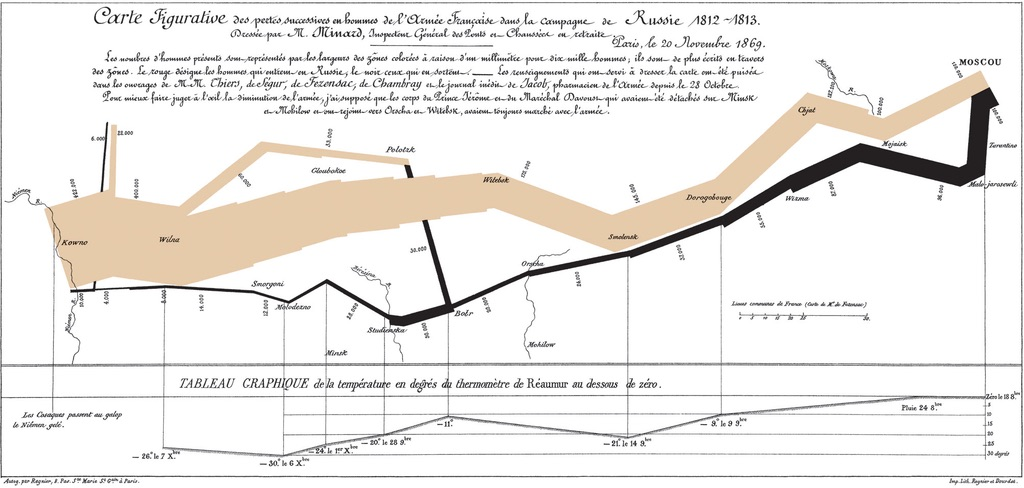
\includegraphics[width=0.75\linewidth]{images/minard-napoleon-march} 

}

\caption{Snow's map shows cholera cases in London during the 1854 epidemic. Taken from https://commons.wikimedia.org/wiki/File:Minard.png (Charles Minard (1781-1870), Public domain, via Wikimedia Commons)}\label{fig:unnamed-chunk-1}
\end{figure}

\hypertarget{napoleons-march}{%
\subsection{Napoleon's March}\label{napoleons-march}}

Napoleon's Russian campaign of 1812, after initial French successes, ended in one of the greatest military disasters in history. The French engineer Charles Minard (1781-1870) illustrated the disastrous outcome of Napoleon's failed Russian campaign. The graph (see Figure XXX) shows the size of the army by the width of the band across the map of the campaign on its outward and return legs, with the temperature on the retreat shown in the line graph below.

The graph starts at the Polish-Russian boarder in June 1812 by showing a thick tan band exhibiting the size of the Grand Army (422,000 men).The width of the line shows the size of the army at each place on the map. In September 1812 the army reached Moscow with 100,000 men. A darker lower band shows the retreat of the Grand Army. This lower band is also linked to temperature scale and dates at the bottom of the chart. It was a bitterly cold winter and the graphic shows the challenges of crossing rivers. Only 10,000 men arrived finally in Poland.

Minard's visualizations tell a story with multivariate data including the size of the army, its location on a two-dimensional surface, direction of the army's movement, and the temperature on various dates during the retreat from Moscow.

Many consider Minard's original to be the best statistical graph ever drawn.

\begin{figure}

{\centering 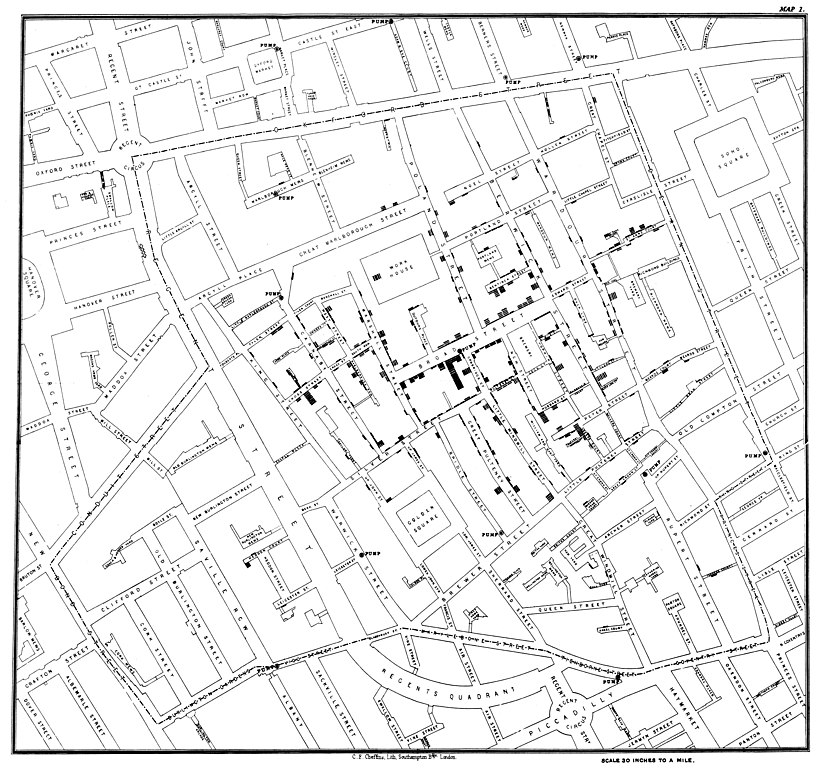
\includegraphics[width=0.75\linewidth]{images/snow-cholera-map} 

}

\caption{Snow's map shows cholera cases in London during the 1854 epidemic. Taken from https://commons.wikimedia.org/wiki/File:Snow-cholera-map-1.jpg (John Snow, Public domain, via Wikimedia Commons)}\label{fig:unnamed-chunk-2}
\end{figure}

\hypertarget{cholera-epidemic-in-london}{%
\subsection{Cholera Epidemic in London}\label{cholera-epidemic-in-london}}

Cholera broke out in Broad Street, London, on the evening of August 31, 1854. This outbreak was one of the most severe outbreaks of cholera in London. One of the investigators of this outbreak, John Snow, suggested that water from the municipal pumps may have caused these deaths. Further investigation of the recorded deaths revealed a strong link between cholera and the Broad Street pump. This pump handle was removed by the authorities after being informed by Snow. How did he arrive at his conclusion and could end the epidemic?

In his book `'Visual Explanation'' Edward R. Tufte \citep{tufte1997visualexplanation} traced Snow's investigation. He highlights that Snow had a hypothesis, `'a causal theory about how the disease spread''. Snow developed this hypothesis from medical analysis and empirical observation. Tufte describes Snow's method by four characteristics. First of all, Snow placed the data in an appropriate context for assessing cause and effect. For this, he created lists ordered by the data of death with the victim's name and the circumstances of their death. However, plotting a time series would not support his reasoning, thus he decided to use a map. He marked the deaths from cholera by black rectangles and existing pumps by black circles with a white corona. Based on this map, Snow could show determine a relation between cholera and the proximity to the Broad Street pump. Second, Snow also made quantitative comparisons, for getting the whole image, he also investigated who escaped the disease. For this, he interviewed people at tow sides - the workhouse and the brewery. As opposed to the neighborhood, no or little deaths were reported. The workhouse had its own pump, and the employees in the brewery were allowed to drink beer. Third, Snow also thought about alternative explanations and contrary cases, thus, Snow traced deaths of people with no obvious link to the Broad street pump. In a number of cases, he could make connections to these cases and the Broad street pump. Finally, Snow assessed possible errors in the reported numbers, thus, he disclosed how he collected or received the data, and discussed possible deficiencies.

Snow's study was a major event in the history of public health and the founding event of the science of epidemiology.

\begin{figure}

{\centering 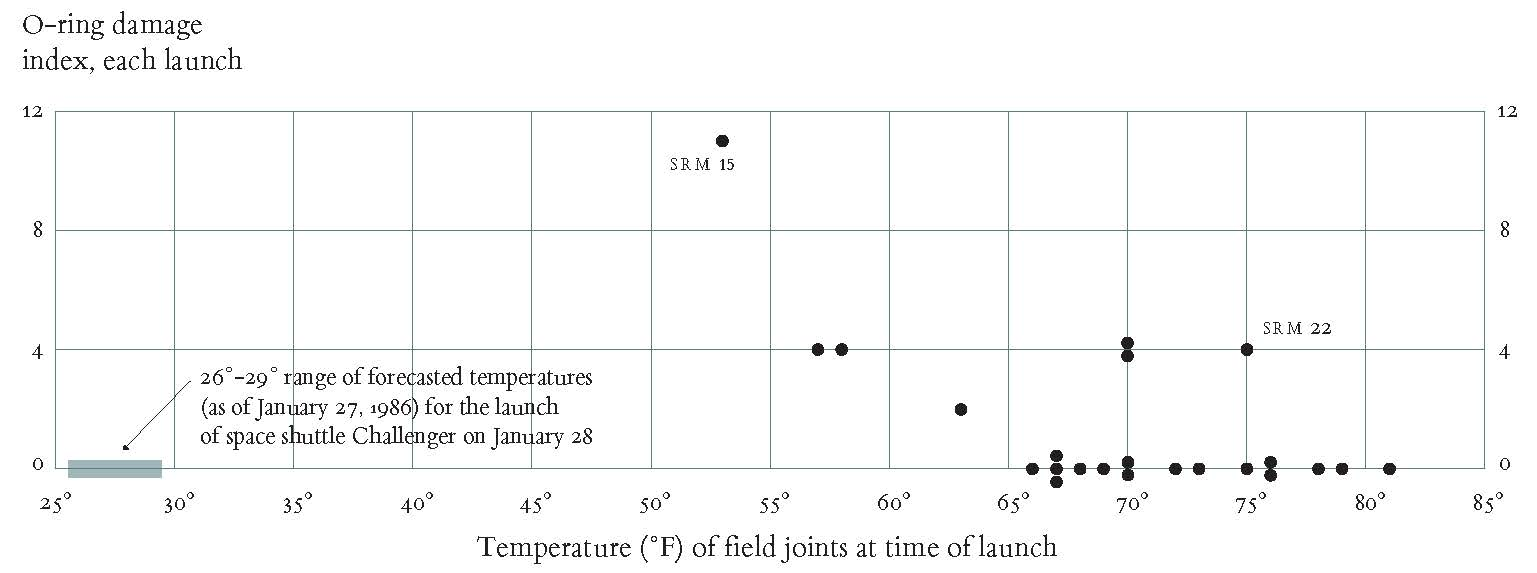
\includegraphics[width=1\linewidth]{images/tufte_challenger_o-ring} 

}

\caption{Snow's map shows cholera cases in London during the 1854 epidemic. Taken from https://commons.wikimedia.org/wiki/File:Snow-cholera-map-1.jpg (John Snow, Public domain, via Wikimedia Commons)}\label{fig:unnamed-chunk-3}
\end{figure}

\hypertarget{space-shuttle-challenger-disaster}{%
\subsection{Space Shuttle Challenger Disaster}\label{space-shuttle-challenger-disaster}}

On January 28, 1986 the Space Shuttle Challenger broke apart shortly after the launch and all seven crew members were killed. Tufte \citep{tufte1997visualexplanation} argues that based on the data provided informed decision making was impossible. Even though, engineers sent 13 charts to the NASA to stop the launch, the provided evidence was inconclusive. They had the correct theory but were not able to display this theory in an understandable way, thus, the correlation between temperature and O-ring distress was not clearly communicated. Instead of analyzing and showing the data of all previous shuttle launches, they considered only selected data. Tufte highlights that instead of focusing on selected data the full range should be considered, especially in cases where the database is rather limited (24 launches prior to Challenger). In their 13 charts, the engineers were not able to convey the existing evidence. It seemed an understanding of the basic principles for effectively communicating data using visualization was missing and this missing understanding led to an incorrect decision. Tufte shows his proposal for an alternative visualization by a graph shown in Figure XX. It is obvious from the data that a launch at 29 degree F is very risky.

In summary, Tufte calls for both the reasoning about statistical evidence and for the design of visualizations and defines six requirements ``(1) \emph{documenting} the sources and characteristics of the data, (2) insistently enforcing appropriate \emph{comparisons}, (3) demonstrating mechanisms of \emph{cause and effect}, (4) expressing those mechanisms \emph{quantitatively}, (5) recognizing the inherently \emph{multivariate} nature of analytic problems, and (6) inspecting and evaluating \emph{alternative explanations}.'' \citep{tufte1997visualexplanation}. Visualizations should be ``documentary, comparative, causal and explanatory, quantified, multivariate, exploratory, skeptical.''\citep{tufte1997visualexplanation}.

\hypertarget{sec:hcd}{%
\section{Human-Centered Data Visualization}\label{sec:hcd}}

Human-Centered Design (HCD) is an approach to systems design and development that aims to make interactive systems more usable by focusing on the use of the system and applying usability knowledge and techniques \citep{international2010ergonomics}. We use the term ``human-centered design'' rather than ``user-centered design'' in order to emphasize that system design can also impact ``indirect'' stakeholders, not just users as ``direct'' stakeholders. However, in practice, these terms are often used synonymously.

The norm provides requirements and recommendations for human-centered design principles and activities throughout the life cycle of computer-based interactive systems, i.e., interactive visualization systems. There are a number of key principles that are defined by a norm of the international standard organization \citep{international2010ergonomics}. The design is based upon an explicit understanding of stakeholders, tasks and environments, thus, the design addresses the whole user experience, i.e., considers the whole context. These stakeholders are, therefore, involved throughout design and development. The iterative design process is driven and refined by human-centered evaluation. The design team includes multidisciplinary skills and perspectives.

HCD comprises a number of dimensions \citep{KlingStar1998_HCD} that can be used for designing data visualizations: (1) Who does the usage of visualization affect? (\emph{stakeholder}); (2) whose purposes are served in the design process and whose not? (\emph{purpose}); and (3) how will the design of the visualization impact people's experience? What unintended consequences might result from the design and the deployment of the visualization? (\emph{context}).

These dimensions can be translated into a process that consists of seven phases.

\hypertarget{the-process-of-visualizing-data}{%
\chapter{The Process of Visualizing Data}\label{the-process-of-visualizing-data}}

In Chapter \ref{sec:introduction}, we have learned that visualization have helped people from the beginning to make sense of their environment. Before we dive deeper into data visualization, we need to build the necessary methodological foundation. For this, we already introduced human-centered design (see Section \ref{sec:introduction}); however, in this chapter, I want to focus specifically on the process of visualizing data. In general, we can differentiate two motivations for visualization design: a problem-driven and a technique driven design \citep{munzner2014visualization}. In the former case, a visualization designer tackles a real-world problem of specific users and attempt to design a solution that helps them work more effectively. Such problem can often be solved based on existing visual encoding and interaction idioms (see Section \ref{sec:hcd}, thus, the main challenge is to understand the problem and translate it into an effective visualization design. In the latter case, a visualization designer has an idea for a new visual encoding, an interaction idiom, or a new algorithm. Sometimes, such ideas emerges during problem-driven visualization design.

\hypertarget{the-process-of-visualizing-data-1}{%
\section{The Process of Visualizing Data}\label{the-process-of-visualizing-data-1}}

When preparing a data visualization project, we are often wondering where to begin with in the first place? From data collection, cleaning, exploration, analysis and visualization, there is a lot that needs to be done in order to derive an insight from data. As you can imagine, there are many proposed data visualization pipelines (e.g., \citep{fry2008visualizing}, \citep{kirk2019data}). However, I would like to focus on one proposition - the four levels nested model of visualization design \citep{munzner2014visualization}. Munzner proposed to divide the problem of visualization design into four cascading levels: (1) the situation level, which contains details of a specific application domain; (2) the data/task abstraction level, where the domain-specific problems and data are separated from context; (3) the visual encoding/interaction idiom level, where the data are visualized and interaction is added; (4) the algorithmic level, where the algorithm is realized to computationally instantiate these idioms. These levels are nested, which means that if you make a bad choice in the abstraction phase, then even perfect choices at the idiom and algorithm levels will not result in a visualization solution that solves the intended problem. For example, you misunderstand the context, and thus, the needs of your stakeholders, because of that you are focusing on the wrong data that are being visualized with a insufficient idiom. Finally, it could happen that your code is too slow. Visualization design is usually a highly iterative refinement process, in other words, visualization design follows the principle of design as redesign. In the following, I detail each of these levels.

The question arises, how you can tackle these challenges properly. Munzner proposes here an immediate validation and downstream validation, in other words, she recommends to properly reflect on each stage on your design decisions before your enter the next level. Taking this very validation-centered perspective on vis design and if you consider that the design of visualizations follows the principle of design as redesign, then your see the parallels to the human-centered design process. You can easily map the Munzner's levels on the HCD process, which makes it easier to position all the methods you already know in Munzner's model.

\hypertarget{the-situation-level}{%
\subsection{The situation level}\label{the-situation-level}}

The \textbf{Domain Situation} contains the details of a specific application domain. This level focuses on a specific domain situation, which encompasses a group of target users, their domain of interest, their questions, and their data. A domain relates to a particular field of interest of the target users of a vis tool, for example open access, microbiology, or health care. Each domain usually has its own vocabulary for describing its data and problems, and there is usually some existing workflow of how the data is used to solve their problems. A group of target users can be narrowly defined as a handful of people working at a specific company, or broadly defined as anybody who does research.

\textbf{Domain Validation} Primary threat is the mischaracterizing of the the problem
An immediate form of validation is to interview and observe the target audience to verify the characterization. Contextual inquiry is typically better suited for vis designers than silent observation because of the complex cognitive tasks that are targeted.
One downstream form of validation is to report the rate at which the tool has been adopted by the target audience. A tool that is actually used by its intended users has reached a different level of success than one that has only been used by its designers.

\hypertarget{the-datatask-abstraction-level}{%
\subsection{The data/task abstraction level}\label{the-datatask-abstraction-level}}

The \_Data/Task Abstraction\_\_ (What-why-level) separates the domain-specific problems and data from the context.
Your goal is to determine which data type would support a visual representation that addresses the user's problem.
Abstracting specific domain questions and data into a domain-independent vocabulary. It allows you to identify situations that are similar, even though there are using a very different language.
Questions from very different domain situations can map to the same abstract vis tasks. We talked about abstract tasks such as browsing, comparing, and summarizing. The data abstraction level requires you to consider whether and how the same dataset provided by a user should be transformed into another form.

\textbf{Abstraction Validation}
The main thread is that the identified task and designed data abstraction do not solve the characterized problems.
A immediate validation is that the system must be tested by target users, rather than doing an abstract task specified by the vis system developers.
A common downstream form of validation is to have a member of the target user community try the tool in controlled user studies. A more rigorous validation approach for this level is to conduct a field study.
Other evaluation methods for visualizations focus on data insight (types of insight visualizations provide and the time it takes to acquire it).

\hypertarget{the-visual-encodinginteraction-idiom-level}{%
\subsection{The visual encoding/interaction idiom level}\label{the-visual-encodinginteraction-idiom-level}}

The \textbf{Visual Encoding/Interaction Idiom} maps the data and task on a visual coding and adds interaction capabilities.
Decision on a specific way to create and manipulate the visual representation of the abstract data, guided by the abstract tasks that you also identified. There are two major concerns at play with idiom design: (1) How to create a single picture of the data? It defines the visual encoding idiom controls exactly what users see. (2) How to manipulate that representation dynamically? The interaction idiom controls how users change what they see.

\textbf{Idiom Validation}
Threat is that the chosen idioms are not effective at communicating the desired abstraction to the person using the system.
One immediate validation approach is to justify the design of the idiom with respect to known perceptual and cognitive principles by using heuristic evaluation or expert reviews. Downstream validation approaches are
* a controlled experiment in a laboratory setting: Evaluating the impact of specific idiom design choices by measuring human performance on abstract tasks or getting qualitative feedback;
* presentation of and qualitative discussion of results in the form of still images or videos as usage scenarios; and
* quantitative measurement of result images (e.g., number of edge crossings in networks.

\hypertarget{the-algorithmic-level}{%
\subsection{The algorithmic level}\label{the-algorithmic-level}}

The \textbf{Algorithm} translates the idioms in a concrete programming language. The level involves all of the design choices involved in creating an algorithm. The goal is to efficiently handle the visual encoding and interaction idioms. The nested model emphasizes separating algorithm design, where your primary concerns are about computational issues, from idiom design, where your primary concerns are about human perceptual issues. There is an interplay between these levels. For example, a design that requires something to change dynamically when the user moves the mouse may not be feasible if computing that would take minutes or hours instead of a fraction of a second.

\textbf{Algorithm Validation} The primary threat is that the algorithm is suboptimal in terms of time or memory performance, either to a theoretical minimum or in comparison with previously proposed algorithms.
An immediate form of validation is to analyze the computational complexity of the algorithm.
The downstream forms of validation:
* Measure the wall-clock time and memory performance of the implemented algorithm
* Determine what data you should use to test the algorithm (use benchmarks)
* Verify the correctness of the algorithm whether through careful testing or formal methods.

\hypertarget{validity-of-your-vis-design}{%
\subsection{Validity of Your Vis Design}\label{validity-of-your-vis-design}}

We differentiate three types of validity: construct validity, internal validity, and external validity.

For example, if a hypothesis states that `'self-esteem'' increases with age, research tracking self-esteem over time from social media must ask whether its assessment of self-esteem from text is actually measuring `'self-esteem'' versus other related or unrelated constructs. In other words, are the observed behaviors (such as words used or frequency of posting) driven primarily by self-esteem as opposed to community norms, variations in system functionality, or other individual aspects.

Internal validity or does our analysis correctly lead from the measurements to the conclusions of the study? For example, an analysis of whether self-esteem increases with age may not be internally valid if data cleaning accidentally removes messages expressing confidence; or if machine learned classifiers were inadvertently trained to recognize self-esteem only in younger people. Of course, while we do not dwell on them, researchers should also be aware of more blatant logical errors---e.g., comparing the self-esteem of today's younger population to the self-esteem of today's older population would be consistent with but would not actually prove that self-esteem increases with age.

For example, effects observed on one social media platform may manifest differently on another platform due to platform differences, differing community or cultural norms. This concept includes what is sometimes called ecological validity, which captures the extent to which an artificial situation (constrained social media platform) properly reflect a broader real-world phenomenon. For example, even after we conclude a successful study of self-esteem in a longitudinal social media dataset, its findings may not generalize to a broader setting because of worries that the kinds of people who self-select into a particular platform are not representative of the broader setting; or that the behaviors they express online may not be representative of their behaviors in other settings.

Each type of Validity has a tradeoff depending on the method applied (see Figure XX).

\begin{figure}

{\centering 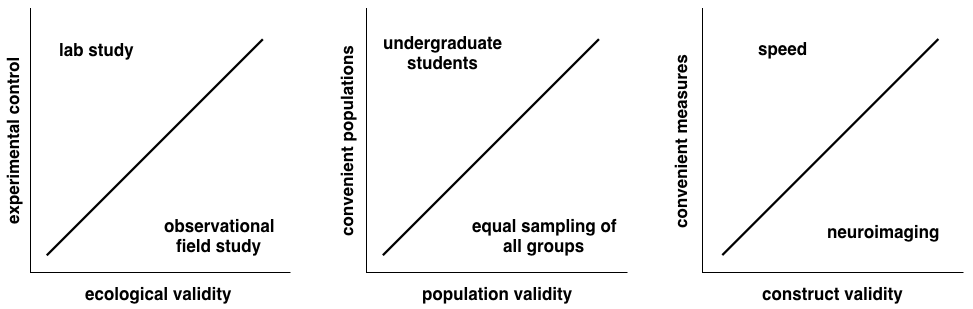
\includegraphics[width=1\linewidth]{images/tradeoff_validity} 

}

\caption{Types of Validity and Tradeoff. Taken from (Padilla, 2018)}\label{fig:unnamed-chunk-4}
\end{figure}

\hypertarget{mapping-the-human-centered-design-process-and-the-nested-model}{%
\section{Mapping the Human-Centered Design Process and the Nested Model}\label{mapping-the-human-centered-design-process-and-the-nested-model}}

In Section \ref{sec:hcd}, we introduced the human-centered design process; how can we bring the nested model and the human-centered design approach together? We can map the analysis step onto the domain situation level, the idea/concept step onto the data/task abstraction level, the design prototype step onto visual encoding/interaction idiom level and the algorithmic level. What is the advantage of this mapping? We can apply all methods, we know from human-centered design for designing our visualizations.

In her visualization design work, Munzner realized that different ways to get a visualization design wrong \citep{munzner2014visualization}. You might identify the wrong problem, by misunderstanding user's needs. You might focus on the wrong data and tasks, thus, you're showing them the wrong thing. You might decide for the wrong idiom, thus, the way you show the data doesn't work. Finally, you might implement the visualization correctly, thus your code is too slow.

\hypertarget{major-elements-of-visualization-design}{%
\section{Major Elements of Visualization Design}\label{major-elements-of-visualization-design}}

In the following, we want to focus on the major elements of visualization design the what--why--how questions which translate into a data--task--idiom trio. By focusing on this trio, we need to answer the following questions:
* What data is shown in the views?
* Why is the task being performed?
* How is the vis idiom constructed in terms of design choices?

In the following, we look into each question in more detail.

\hypertarget{reflecting-on-data}{%
\subsection{Reflecting on Data}\label{reflecting-on-data}}

Back in 2017, the newspaper `'The Economist'' published a story titled, ``The world's most valuable resource is no longer oil, but data.'' Since its publication, the topic has generated a great deal of discussion, and ``Data is the new oil'' has become a common refrain. How could this happen?

Already in 2008, the Wired magazine editor Chris Anderson titled in an article ``The End of Theory,'' (\url{https://www.wired.com/2008/06/pb-theory/}).

\begin{quote}
This is a world where massive amounts of data and applied mathematics replace every other tool that might be brought to bear. Out with
every theory of human behavior, from linguistics to sociology. {[}\ldots{]} Who knows why people do what they do? The point is they do it, and we \textgreater{} can track and measure it with unprecedented fidelity. With enough data, the numbers speak for themselves.

--- Chris Anderson, WIRED, 2008
\end{quote}

Anderson made the claim that ``with enough data, the numbers speak for themselves.'' The article explains several examples of how the abundance of data helps people and companies take decision without even having to understand the meaning of the data itself. His assertion was that the age of Big Data will soon permit data scientists to do analysis at the scale of the population. Statistics is based on the idea that you can infer things about a population by taking a random and representative sample.At the point when we have data collected about an entire population, theory is no longer necessary. We also, he wrote, don't need models and theories to understand why something is happening, just to be able to see that one thing is correlated with another: ``Correlation is enough.''

As D'Ignazio and Klein \citep{dignazio2020datafeminism} point out, there is a misconception when saying that `'numbers speak for themselves''. The assumption is that data are a raw input rather than seeing them as artifacts that have emerged ``fully cooked'' into the world, birthed out of a complex set of social and political circumstances already existing in the data setting. But data is an output first. After that, it can become an input into a new process, but only with understanding of what the limitations of the collection environment were. ``Raw Data'' is an Oxymoron. Many data-driven projects aiming towards producing new, future insights forget to interrogate how the data got collected and cooked in the first place.

What is the difference between data, information, and knowledge?

The following three points summarize the essential differences between the three concepts \citep{aamodt1995datainformationknowledge}:
Data are syntactic entities, i.e., data are patterns with no meaning; they are input to an interpretation process, i.e.
to the initial step of decision making. Information is interpreted data, i.e., information is data with meaning; it is the output from data interpretation as well as the input to, and output from, the knowledge-based process of decision making. Knowledge is learned information, i.e., knowledge is information incorporated in an agent's reasoning resources, and made ready for active use within a decision process; it is the output of a learning process. The role of knowledge, in general, is therefore to play the active part in the processes of transforming data into information, deriving other information, and acquiring new knowledge, i.e., to learn. This leads to the following summary of knowledge roles: knowledge is needed to transform data into information; knowledge is needed to derive new information from existing; knowledge is needed to acquire new knowledge, thus is referred to as data interpretation, to as elaboration, and to as learning.

As Donna Harraway emphazised all knowledge is `'situated.'' \citep{haraway1988situated} It means that context matters. When we want to create new knowledge based on a given dataset, we have to reflect about the social, cultural, historical and material conditions in which that data was produced, as well as the people who created that data.Rather defining data as objective, that can be taken as it is, we need to connect data back to their context, to better understand existing limitations, but also for example, ethical obligations, or existing privacy concerns. However, we also need to think about our own role when analyzing the data. What is our perspective we bring in and how we decide which part of the data are valuable and which don't. To come back to Chris Anderson. His post was possible also a provocation but when working with data, we need \emph{more} theory, context, and scientific methods, not less. Why? Because data is often created by humans or by software that was designed by humans. Thus, it makes sense to add qualitative data to a dataset.

Thick Data or qualitative data is data brought to light using qualitative, ethnographic research methods that uncover people's emotions, stories, and models of their world \citep{wang2016bigdata}. It's the sticky stuff that's difficult to quantify. It comes to us in the form of a small sample size and in return we get an incredible depth of meanings and stories. Thick Data is the opposite of Big Data (or thin data), which is quantitative data at a large scale that involves new technologies around capturing, storing, and analyzing. For Big Data to be analyzable, it must use normalizing, standardizing, defining, clustering, all processes that strips the the data set of context, meaning, and stories. Thick Data can rescue Big Data from the context-loss that comes with the processes of making it usable.

Big Data requires a humongous N to uncover patterns at a large scale while Thick Data requires a small N to see human-centered patterns in depth. Both types of Thick Data relies on human learning, while Big Data relies on machine learning. Thick Data reveals the social context of connections between data points while Big Data reveals insights with a particular range of quantified data points. Thick Data techniques accepts irreducible complexity, while Big Data techniques isolates variables to identify patterns. Thick Data loses scale while Big Data loses resolution.

Thus it makes sense to take a human-centered design approach. You should think about the audience, the purpose and the context of your research.
* Audience: Who are you publishing your research for?
* Purpose: How do you want them to use your research?
* Context: What factors (under your control) will impact whether/how they use it?

Publishing your research openly shows that you take responsibility for your research. Including the possibility that you might be wrong. It provides transparency around your values, motivations, and assumptions. Having a public audience in mind when designing and publishing your projects encourages you to reflect on your values, motivations, assumptions, and thought process---and how that might influence your project. Thinking in terms of HCD can also help you think of trade-offs in open research. For example, it can help you decide when/what NOT to publish openly!

\hypertarget{data-set}{%
\subsubsection{Data Set}\label{data-set}}

What kind of data are you given? What information can you figure out from the data, versus the meanings that you must be told explicitly? What high-level concepts will allow you to split datasets apart into general and useful pieces? To move beyond guesses, you need to know two crosscutting pieces of information about these terms: their semantics and their types. The semantics of the data is its real-world meaning.

A dataset is any collection of data. There are four basic dataset types: tables, networks/trees, spatial (fields, geometry). In real-world situations, complex combinations of these basic types are common.

Consider the concept of a table as a type of record that is independent of any particular visual representation. In (simple flat) tables, each row represents an item of data, and each column is an attribute of the dataset. Each cell in the table is fully specified by the combination of a row and a column and contains a value for that pair. A multidimensional table has a more complex structure since each cell is indexed by multiple keys. It can be a table in a table, which is called a tensor.

Networks are well suited for specifying some kind of relationship between two or more items. An item in a network is often called a node (or vertex). A link (or edge) is a relation between two items. Nodes can have associated attributes, just like items in a table.Links could also have attributes associated with them; these may be partly or wholly disjoint from the node attributes. Networks can also be represented by two tables. Networks with hierarchical structure are more specifically called trees. In contrast to a general network, trees do not have cycles: each child node has only one parent node pointing to it.

The field dataset type also contains attribute values associated with cells. Each cell in a field contains measurements or calculations from a continuous domain. Continuous phenomena include temperature, pressure, speed, force, and density (or mathematical functions).
Continuous data requires careful treatment that takes into account the mathematical questions of sampling, how frequently to take the measurements, and interpolation, how to show values in between the sampled points in a way that does not mislead.

The geometry dataset type specifies information about the shape of items with explicit spatial positions. The items could be points, or one-dimensional lines or curves, or 2D surfaces or regions, or 3D volumes. Spatial data often includes hierarchical structure at multiple scales.

\hypertarget{what-data-types-should-be-differentiated}{%
\subsubsection{What Data Types Should be Differentiated?}\label{what-data-types-should-be-differentiated}}

An attribute is some specific property that can be measured, observed, or logged. For example, attributes could be salary, price, or protein expression levels.
An item is an individual entity that is discrete, such as a row in a simple table. For example, items may be people, stocks, or genes.
A link is a relationship between items, typically within a network.\\
A position is spatial data, providing a location in two-dimensional (2D) or three-dimensional (3D) space.
A grid specifies the strategy for sampling continuous data in terms of both geometric and topological relationships between its cells.

\hypertarget{sec:variabletype}{%
\subsubsection{What Attribute Types Do you Know?}\label{sec:variabletype}}

What kind of data are you given? What information can you figure out from the data, versus the meanings that you must be told explicitly? What high-level concepts will allow you to split datasets apart into general and useful pieces?

To move beyond guesses, you need to know two crosscutting pieces of information about these terms: their semantics and their types. The semantics of the data is its real-world meaning.

\begin{figure}

{\centering 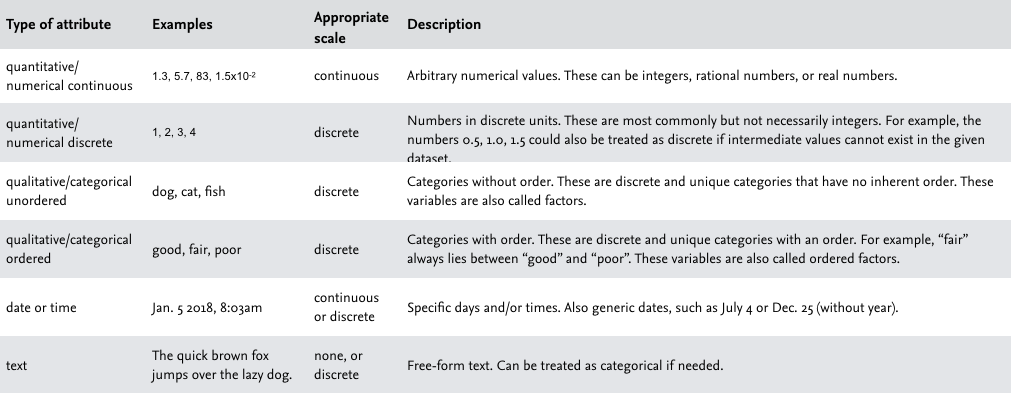
\includegraphics[width=1\linewidth]{images/attribute_types} 

}

\caption{Types of variables encountered in typical data visualization scenarios. Taken from (https://clauswilke.com/dataviz/aesthetic-mapping.html)}\label{fig:unnamed-chunk-5}
\end{figure}

\hypertarget{reflecting-on-tasks}{%
\subsection{Reflecting on Tasks}\label{reflecting-on-tasks}}

Why Analyze Tasks Abstractly? You need to consider tasks in an abstract form, rather than the domain-specific way that users typically think about them. Transforming task descriptions from domain-specific language into abstract form allows you to reason about similarities and differences between them.

Munzner \citep{munzner2014visualization} differentiated a small set of carefully chosen words to describe why people are using visualization, designed to help you crisply and concisely distinguish between different goals. We differentiate a set has verbs describing actions, and nouns describing targets.

\hypertarget{user-goals-are-defined-by-actions}{%
\subsubsection{User Goals are Defined by Actions}\label{user-goals-are-defined-by-actions}}

We can define three levels of action. The high-level choices describe how the visualisation is being used to analyze, either to consume existing data or to also produce additional data. The mid-level choices cover what kind of search is involved, in terms of whether the target and location are known or not. The low-level choices pertain to the kind of query: does the user need to identify one target, compare some targets, or summarize all of the targets? Decisions at each of these three levels are independent, and it is usually useful to describe actions at all three levels.

\emph{Action: Analyze for Consumption or Production} In contrast to the use of vis only for the consumption of existing information, in the production case the intention of the user is to generate new material. Often, the goal in production is to produce output that is immediately used as input for a next instance. Sometimes the user intends to use this new material for some other vision-related task, such as discovery or presentation. Sometimes the intended use of the new material is for another purpose that does not require a vis, such as downstream analysis with non-visual tools. There are three types of production goals: Annotate, Record, and Derive.

\emph{Action: Search and their Classification} All high-level analysis cases require the user to search for items of interest within the vis as a middle-level target. The classification of search into four alternatives is broken down according to whether the identity and location of the search target is already known or not. If users already know both what they're looking for and where it is, then the search type is simply lookup. If users want to find a known target at an unknown location, the search type is locate, that is, find out where the specific object is. If users don't know exactly what they're looking for, but they do have a location in mind of where to look for it, the search type is browse. If users are not even sure of the location, the search type is explore.

\emph{Action: Query}
A low-level user goal is to query targets at one of three scopes. Once a target or set of targets for a search has been found, a low- level user goal is to query these targets at one of three scopes: identify, compare, or summarize. The progression of these three corresponds to an increase in the amount of search targets under consideration: one, some, or all. That is, identify refers to a single target, compare refers to multiple targets, and summarize refers to the full set of possible targets.

\emph{Actions Refer to Targets}
All actions refer to a target, i.e.~an aspect of the data that is of interest to the user. The idea of a goal is explicit in search and query actions. It is more implicitly related to the usage actions, but still relevant: for example, what the user presents or discovers.

Tasks are defined by a \{action, target\} pairs, for example, discover distribution, compare trends, locate outliers, browse topology.

\hypertarget{the-how-of-visualization-design---at-a-glance}{%
\subsection{The How of Visualization Design - At A Glance}\label{the-how-of-visualization-design---at-a-glance}}

Bostock et al. \citep{Heer_Bostock_Ogievetsky_2010} state:

\begin{quote}
All visualizations share a common ``DNA'' -- a set of mappings between data properties and visual attributes
such as position, size, shape, and color -- and customized species of visualizations might always be constructed \textgreater{} by varying these encodings.
\end{quote}

\textbf{More Coming Soon}

\hypertarget{understanding-your-data}{%
\chapter{Understanding your Data}\label{understanding-your-data}}

By building on the Nested odel of Munzner \citep{munzner2014visualization}, we have realized how important it is to understand the context of the data origin and the data at hand. In this chapter, we focus on the data, because many data viz project start with so-called `'found data''. These are data sets that are openly available on the internet, data sets in which creating you were not involved. The increasing use of data everywhere requires to think about data literacy, inclusion, and fairness to ensure that data creates value \citep{KoestenSimperl2021_dataUX}. However, data is often reused, thus, we need to reflect on where data has been created. Koesten \& Simperl \citep{KoestenSimperl2021_dataUX} differentiate three main activities to interact with data: inspecting, engaging with the data, and placing data in context.

Thus, in order to understand, whether data are valuable for your research question and which questions you can really tackle with these data, you need an understanding of its origin (the context of creation) and an understanding of its structure.

\hypertarget{understanding-the-data-context}{%
\section{Understanding the Data Context}\label{understanding-the-data-context}}

People's perception of what constitutes good-quality data changed as they engaged with the data. Koesten \& Simperl \citep{KoestenSimperl2021_dataUX} highlight the importance of engagement around datasets, including discussions, feedback, reviews, ratings, and means to contact data creators. User communities and peer support can complement documentation efforts and make dataset maintenance sustainable. They, furthermore, propose the three activities:

\begin{enumerate}
\def\labelenumi{\arabic{enumi}.}
\tightlist
\item
  Explore the environment of the dataset's creation (e.g., a study setup or the conditions surrounding data collection, with timeframes, geospatial boundaries, or configurations of collection devices).
\item
  Explore the norms of the discipline in which the data was collected, including methods of analysis and validation, as well as limitations (e.g., common margins of error).
\item
  Connect data with the world, gauging how representative it is and reflecting on assumptions about how much it mirrors reality (includes also the question of what might be missing from the data.
\end{enumerate}

Gebru et al. \citep{Gebruetal2018datasheets} propose `'datasheets'' inspired by more robust documentation standards in the electronics industry. Datasheets are meant to improve transparency and accountability of datasets and to be useful to both dataset creators and dataset consumers.
For consumer of datasets, datasheets should encourage reflection on the process of creating, distributing, and maintaining a dataset (including benefits and harms). For dataset creators it helps also to reflect on the data and to make more informed decisions about its use. The authors offer guiding questions towards creating datasheets for datasets:

\begin{itemize}
\tightlist
\item
  Motivations: Describe the motivations for creating the dataset, including funding, any specific tasks the authors had in mind, and who the authors are.
\item
  Composition: Describe the composition of the dataset, like what kinds of data are in it, how it was collected, whether labels are associated with the data, and whether the dataset contains sensitive information.
\item
  Collection Process: Describe the data collection process, like how the data was collected, where or who is was collected from, who was involved in the collection process, and, if people are involved, if consent was given for the data to be collected.
\item
  Processing: Whether the data was process or labelled and how it was done.
\item
  Uses: The tasks the dataset is intended to be used for, how it has already been used, and limitations of use.
  Distribution: How the dataset will be distributed and to who, and any restrictions on distribution.
\item
  Maintenance: Who and how the dataset will be maintained, and if and how others will be able to build on it.
\end{itemize}

Building on this idea Holland et al. \citep{Hollandetal2018DatasetNutritionLabel} proposed the \href{https://datanutrition.org/}{dataset nutrion label}. An example is given in Fugure

\begin{figure}

{\centering 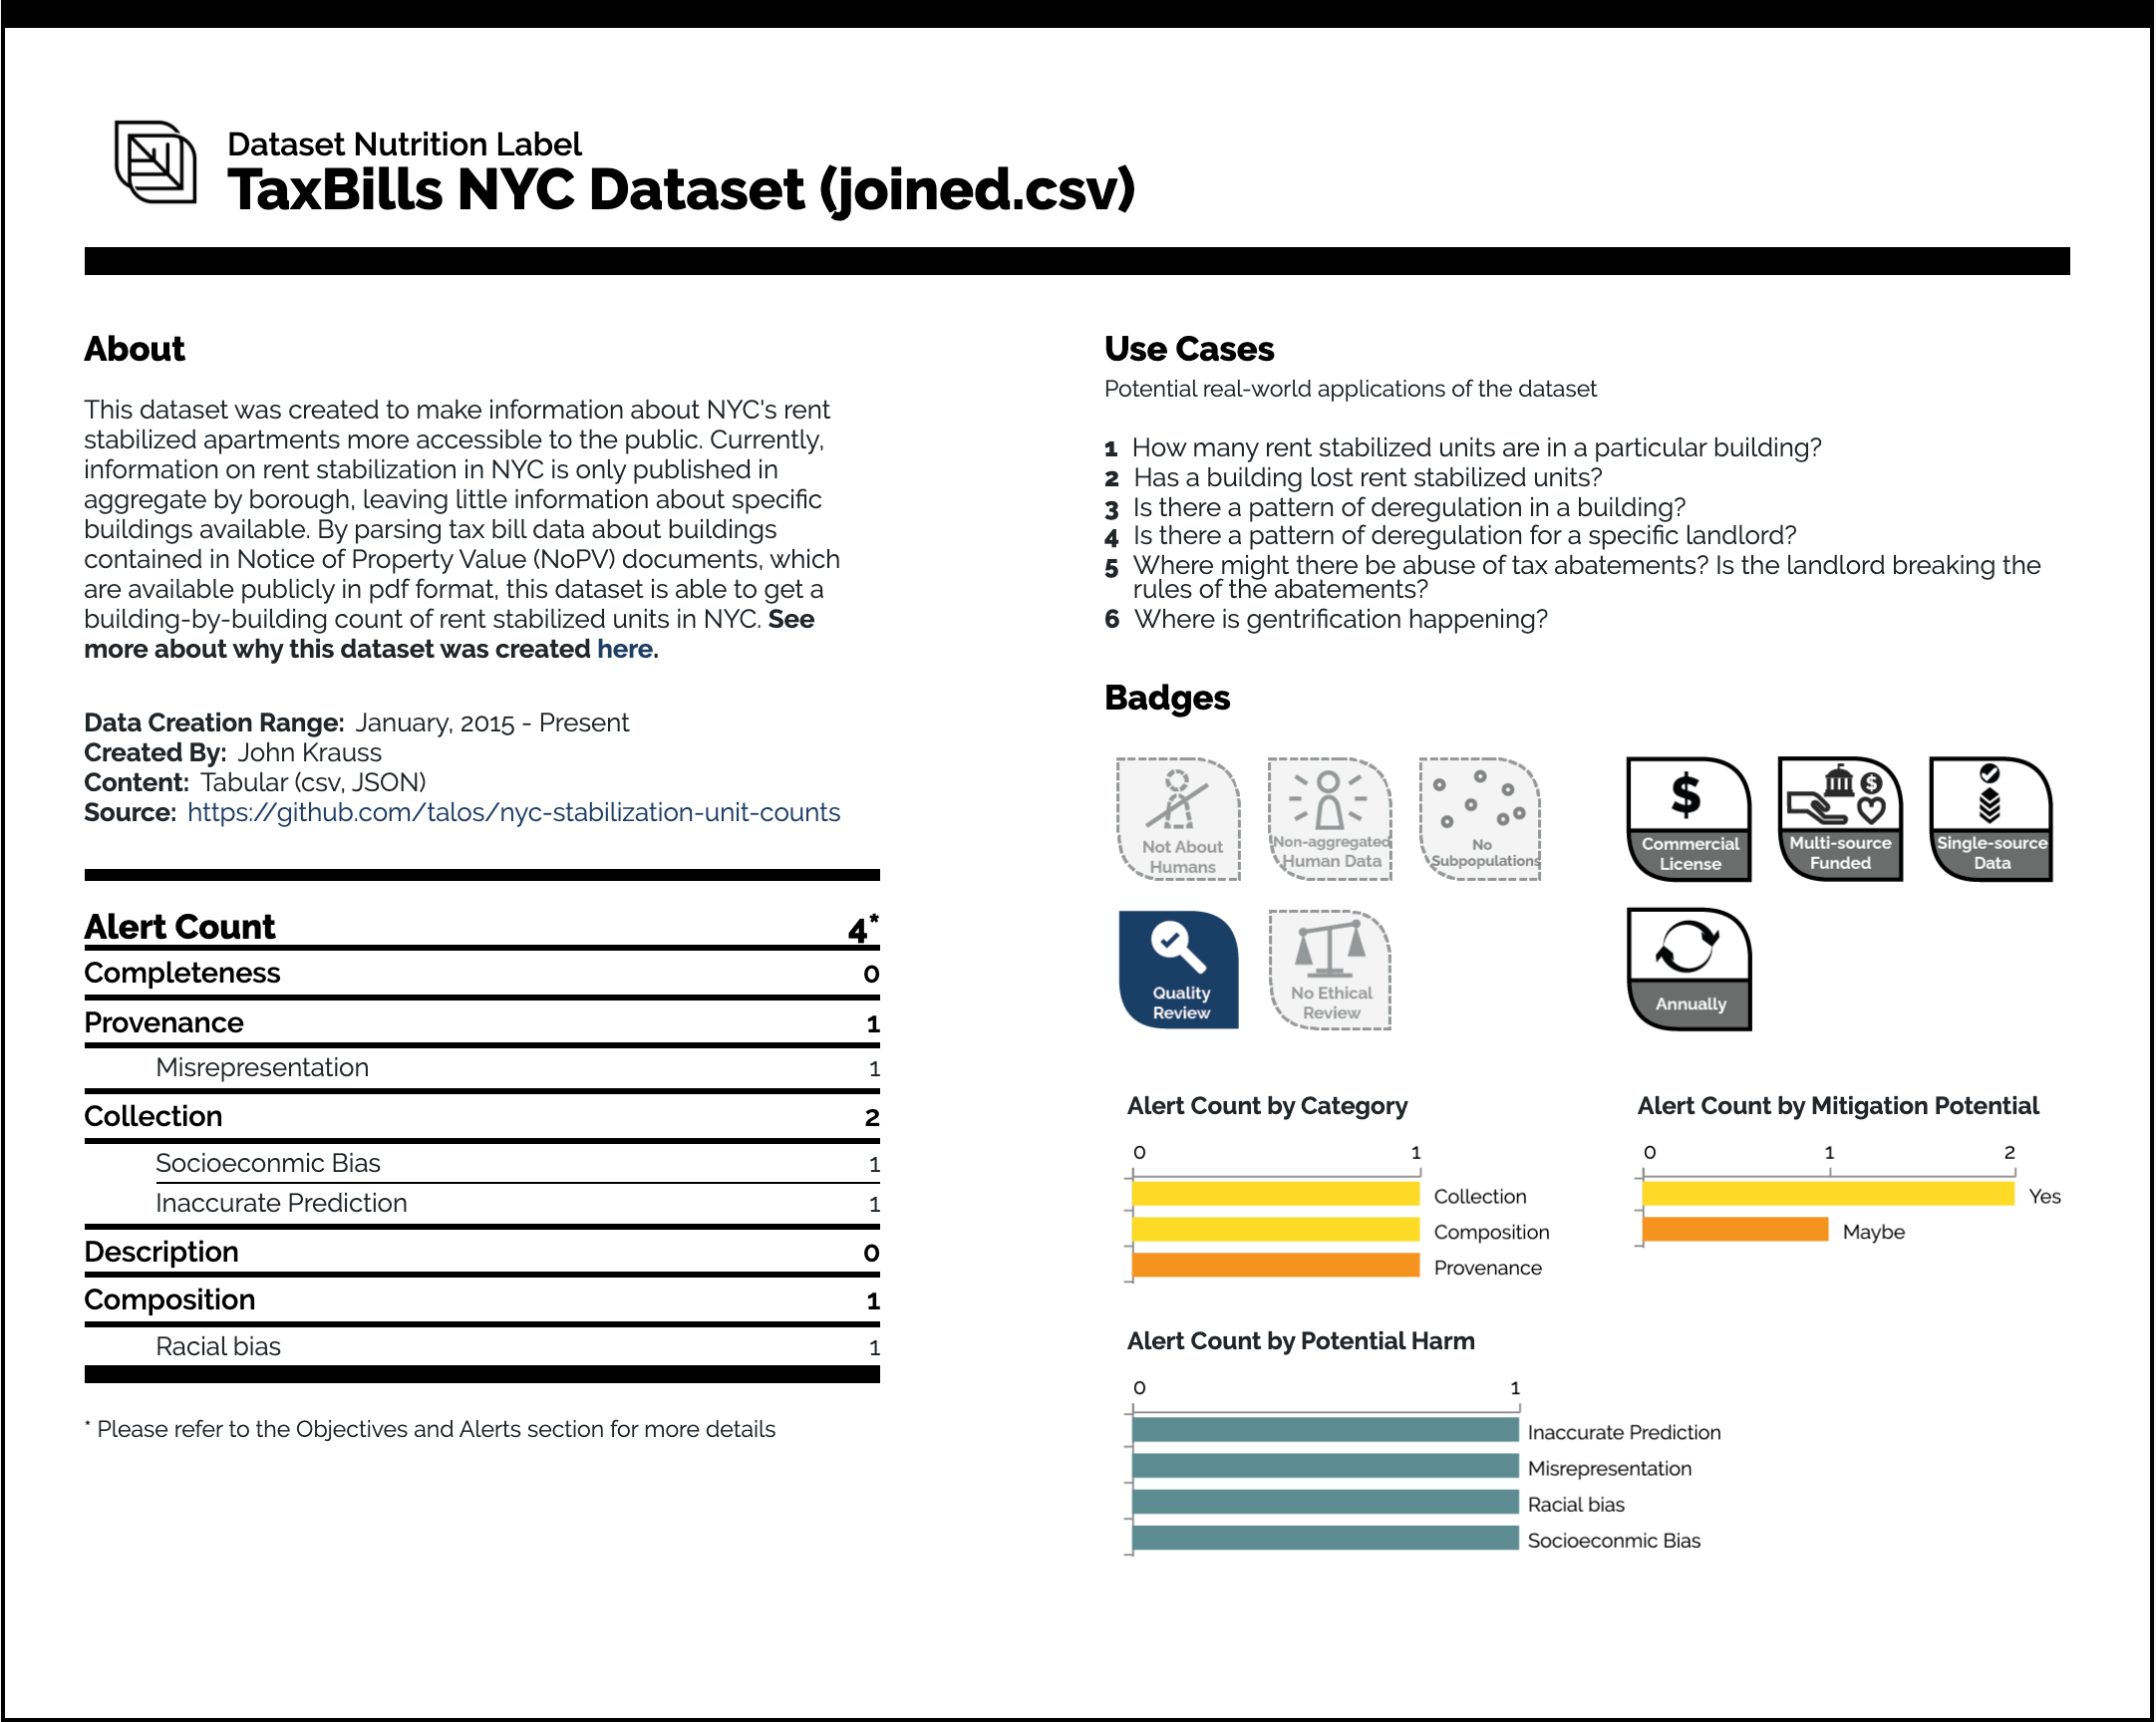
\includegraphics[width=1\linewidth]{images/dataset_nutrion_label} 

}

\caption{Example of the Dataset Nutrion Label (first generation). Taken from https://datanutrition.org/}\label{fig:unnamed-chunk-6}
\end{figure}

\hypertarget{Understanding-the-Data-Structure}{%
\section{Understanding the Data Structure}\label{Understanding-the-Data-Structure}}

In this section, we focus on understanding the structure of our data by employing the Exploratory Data Analysis (EDA). EDA is an approach of analyzing data sets to summarize their main characteristics by using data visualizations. In 1970 John Tukey \citep{Tukey1977eda} introduced EDA with this seminal book on this topic. He was an extraordinary scientist who had a profound impact on statistics and computer science\footnote{I highly recommend reading more about him, for example in \url{https://www.stat.berkeley.edu/~brill/Papers/life.pdf} .}. Much of what we cover in EDA today is based on his work. Part of EDA is the so-called initial data analysis (IDA) (\url{https://towardsdatascience.com/a-basic-guide-to-initial-and-exploratory-data-analysis-6d2577dfc242}). IDA focuses on identifying data inconsistencies (e.g., missing values) and the description of the data properties; thus, EDA encompasses IDA.

EDA allows the data analysts to achieve a richer qualitative understanding by `'looking at data to see what it seems to say''. Explorative Data Analysis should be understood as an iterative process that supports:
* the search for answers by visualizing, transforming, and modeling your data,
* the generation of hypotheses about what might be happening in a data set, and
* the refining of your analysis goals or the generation of additional goals.

This step should not be underestimated since data analysts spend much of their time (sometimes 80\% or more) cleaning and formatting data to make it suitable for analysis, then actually carrying out the analysis.

EDA is based on three principles: (1) Continuous openness and re-expression, (2) Initial skepticism, and (3) Exploratory versus confirmatory. Rather than immediately imposing a model on the data that may obscure important details, EDA analysts try to find patterns in the data and describe them with simple summary statistics (descriptive statistics). It may take several iterations for the analyst to reach a satisfactory summary or `'smoothing'' of the data\footnote{The so-called ``smooth part of a data set'' is the variability that the analyst has accounted for so far, while the ``rough'' part is the variability that remains unexplained.} Re-expressions or transformations of the data are essential for smoothing because they help the analyst identify new patterns.
Because EDA analysts assume that there is no uniquely correct numerical summary of a data set, they are very skeptical of initial numerical summaries. Numerical summaries and smoothings are constantly tested against the raw data to ensure that they adequately represent the data. To identify patterns and look for data points that do not fit the smooth part (outliers), EDA analysts rely heavily on visualization.
By supporting data exploration, EDA helps researchers generate hypotheses. These hypotheses can later be tested with formal confirmatory procedures using inferential statistics.

In summary, your goal during the EDA is to develop an understanding of your data. The easiest way to accomplish this is to use questions to guide your investigation. When you ask a question, the question focuses your attention on a particular part of your data set and helps you decide which graphs, models, or transformations to make.

EDA is a creative process \citep{WickhamGrolemund2017Rfordatascience}, thus the key to asking meaningful questions is to generate a large number of questions. Of course, it is very challenging to generate these questions at the beginning because you are not familiar with the dataset. On the other hand, each new question you ask will expose you to a new aspect of your data and increase your chance of discovery. You can quickly break down the most interesting parts of your data - and develop a thought-provoking set of questions - if you follow each question with a new question based on your findings. This challenge has been already formulated by Tukey:

\begin{quote}
Far better an approximate answer to the right question, which is often vague, than an exact answer to the wrong question,
which can always be made precise.
--- John Tukey (The future of data analysis. Annals of Mathematical Statistics 33 (1), (1962), page 13)
\end{quote}

There is no rule about what questions you should ask to guide your research. However, two types of questions will always be useful for making discoveries in your data. You can phrase these questions loosely as (1) What kind of variation occurs within my variables? and (2) What kind of co-variation occurs between my variables?

\hypertarget{using-r-for-data-exploration}{%
\subsection{Using R for Data Exploration}\label{using-r-for-data-exploration}}

In the following, we address these two questions based on the example of Héctor Corrada Bravo from the EDA chapter of his course on \href{http://www.hcbravo.org/IntroDataSci/bookdown-notes/exploratory-data-analysis-visualization.html}{`'Introduction to Data Science''} from the Center for Bioinformatics and Computational Biology from the Univ. of Maryland.

We employ the GNU R which is a widespread tool for statistical analysis. However, you can follow these steps with any programming language at hand. I would like to provide you an methodological understanding of how to explore data, rather than provide an introduction into R (\url{http://www.r-project.org/}) which is a GNU project, thus, R is Free Software under the terms of GPL. There are over 2,000 user-contributed packages available at R CRAN (\url{https://cran.r-project.org/}) with packages for specific functions or specific areas of study. It has an excellent integration with DBs (MySQL, SQLite) and automation based on scripts is easy. Furthermore, the graphical user interface RStudio (\url{https://www.rstudio.com/}) makes its usage very convenient. R is an interpreted language. It supports procedural programming with functions and, for some functions, object-oriented programming with generic functions. A generic function acts differently depending on the type of arguments passed to it, for example, R has a generic print() function that can print almost every type of object in R with a simple `'print(objectname)'' syntax. A Base R Cheat Sheet can be found \href{https://www.povertyactionlab.org/sites/default/files/r-cheat-sheet.pdf}{here}.

\hypertarget{visualizing-data}{%
\subsection{Visualizing Data}\label{visualizing-data}}

In the following, we use the on-time data for all flights that departed NYC, i.e., JFK, LGA or EWR, in 2013. The Bureau of transportation statistics has released these data, and it was included into R. Let's get an overview about this dataset.

\begin{Shaded}
\begin{Highlighting}[]
\FunctionTok{library}\NormalTok{(nycflights13)}
\FunctionTok{library}\NormalTok{(skimr)}

\CommentTok{\# Show the internal structure of the R object (= flights)}
\FunctionTok{str}\NormalTok{(flights)}
\end{Highlighting}
\end{Shaded}

\begin{verbatim}
## tibble [336,776 x 19] (S3: tbl_df/tbl/data.frame)
##  $ year          : int [1:336776] 2013 2013 2013 2013 2013 2013 2013 2013 2013 2013 ...
##  $ month         : int [1:336776] 1 1 1 1 1 1 1 1 1 1 ...
##  $ day           : int [1:336776] 1 1 1 1 1 1 1 1 1 1 ...
##  $ dep_time      : int [1:336776] 517 533 542 544 554 554 555 557 557 558 ...
##  $ sched_dep_time: int [1:336776] 515 529 540 545 600 558 600 600 600 600 ...
##  $ dep_delay     : num [1:336776] 2 4 2 -1 -6 -4 -5 -3 -3 -2 ...
##  $ arr_time      : int [1:336776] 830 850 923 1004 812 740 913 709 838 753 ...
##  $ sched_arr_time: int [1:336776] 819 830 850 1022 837 728 854 723 846 745 ...
##  $ arr_delay     : num [1:336776] 11 20 33 -18 -25 12 19 -14 -8 8 ...
##  $ carrier       : chr [1:336776] "UA" "UA" "AA" "B6" ...
##  $ flight        : int [1:336776] 1545 1714 1141 725 461 1696 507 5708 79 301 ...
##  $ tailnum       : chr [1:336776] "N14228" "N24211" "N619AA" "N804JB" ...
##  $ origin        : chr [1:336776] "EWR" "LGA" "JFK" "JFK" ...
##  $ dest          : chr [1:336776] "IAH" "IAH" "MIA" "BQN" ...
##  $ air_time      : num [1:336776] 227 227 160 183 116 150 158 53 140 138 ...
##  $ distance      : num [1:336776] 1400 1416 1089 1576 762 ...
##  $ hour          : num [1:336776] 5 5 5 5 6 5 6 6 6 6 ...
##  $ minute        : num [1:336776] 15 29 40 45 0 58 0 0 0 0 ...
##  $ time_hour     : POSIXct[1:336776], format: "2013-01-01 05:00:00" "2013-01-01 05:00:00" ...
\end{verbatim}

The first line shows the dimension of your data frame\footnote{A dataframe is a list, with each component of that list being a equal length vector. Thus, intuitively, a dataframe is like a matrix with a rows-and-comlumns-structure. However, it differs from a matrix, since each column can having different mode (data type) \citep{Matloff2011ArtofRProgramming}.}, and then each of the columns (attributes) and show with their respective datatype.

Understanding the structure of the dataset is quite useful, since it allows you to get an overview on the available data types. A good understanding of the different data types is an important prerequisite for EDA, because you can use certain statistical measurements only for certain data types. You also need to know which data type you are dealing with in order to choose the right visualization method. Think of data types as a way to categorize different types of variables. We already discussed different types of variables in Section \ref{sec:variabletype}.

For setting up the pipeline it makes sense to work with a subset only, thus, we sample from the available data 10 percent. Furthermore, I decided to include only those observations that are complete. However, this decision should not be made carelessly.

\begin{Shaded}
\begin{Highlighting}[]
\FunctionTok{library}\NormalTok{(dplyr)}

\CommentTok{\# Select a sample from the whole data set}
\NormalTok{fly.sample }\OtherTok{\textless{}{-}} \FunctionTok{sample\_frac}\NormalTok{(flights, .}\DecValTok{1}\NormalTok{) }\CommentTok{\# takes a sample of 10 per cent}

\CommentTok{\# dimensions of the data set}
\FunctionTok{dim}\NormalTok{(fly.sample) }
\end{Highlighting}
\end{Shaded}

\begin{verbatim}
## [1] 33678    19
\end{verbatim}

\begin{Shaded}
\begin{Highlighting}[]
\CommentTok{\# remove all observations that are not complete}
\NormalTok{fly.sample }\OtherTok{\textless{}{-}}\NormalTok{ fly.sample[}\FunctionTok{complete.cases}\NormalTok{(fly.sample), ]}

\CommentTok{\# dimensions of the data set}
\FunctionTok{dim}\NormalTok{(fly.sample)}
\end{Highlighting}
\end{Shaded}

\begin{verbatim}
## [1] 32674    19
\end{verbatim}

\hypertarget{scatterplot}{%
\subsection{Scatterplot}\label{scatterplot}}

The next step is to get a first overview about the data, and for this, we can use a visualization already. For this I use a simple scatterplot.

\begin{Shaded}
\begin{Highlighting}[]
\FunctionTok{library}\NormalTok{(ggplot2)}
\FunctionTok{library}\NormalTok{(tibble)}

\CommentTok{\# Visualize Data 1 {-} Scatterplot}
\NormalTok{fly.viz1 }\OtherTok{\textless{}{-}} \FunctionTok{rowid\_to\_column}\NormalTok{(fly.sample)}
\FunctionTok{ggplot}\NormalTok{(fly.viz1, }\FunctionTok{aes}\NormalTok{(}\AttributeTok{x=}\NormalTok{rowid, }\AttributeTok{y=}\NormalTok{dep\_delay)) }\SpecialCharTok{+} \FunctionTok{geom\_point}\NormalTok{() }\SpecialCharTok{+} 
  \FunctionTok{xlab}\NormalTok{(}\StringTok{"Flight ID"}\NormalTok{) }\SpecialCharTok{+} \FunctionTok{ylab}\NormalTok{(}\StringTok{"Departure delay (in min)"}\NormalTok{) }
\end{Highlighting}
\end{Shaded}

\begin{figure}
\centering
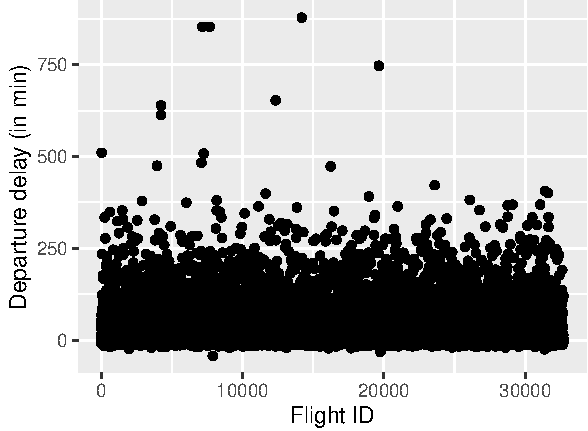
\includegraphics{Human-Centered-Data-Viz_files/figure-latex/chunk-label3-1.pdf}
\caption{\label{fig:chunk-label3}Scatterplot of delay times.}
\end{figure}

This is not very informative because this plot is not structured. However, let us reflect about the visualization for a moment. A scatterplot encodes two quantitative variables using both the vertical and horizontal spatial position channels., and the mark type is necessarily a point. They are highly effective for judging the correlation between two attributes. Scatterplots are often augmented with color coding to show an additional attribute. We talk about these characteristics in detail again.

\begin{longtable}[]{@{}
  >{\raggedright\arraybackslash}p{(\columnwidth - 2\tabcolsep) * \real{0.35}}
  >{\raggedright\arraybackslash}p{(\columnwidth - 2\tabcolsep) * \real{0.65}}@{}}
\caption{Characteristics of a scatterplot \citep{munzner2014visualization}}\tabularnewline
\toprule
Idiom & Scatterplot \\
\midrule
\endfirsthead
\toprule
Idiom & Scatterplot \\
\midrule
\endhead
What: Data & Table: two quantitative value attributes. \\
How: Encode & Express values with horizontal and vertical spatial position and point marks \\
Why: Task & Find trends, outliers, distribution, correlation; locate clusters. \\
Scale & Items: hundreds \\
\bottomrule
\end{longtable}

Let's sort the values and change the graphical representation to make it easier to see.

\begin{Shaded}
\begin{Highlighting}[]
\CommentTok{\# Visualize Data {-} Scatterplot with ordered values}

\CommentTok{\# \textquotesingle{}arrange\textquotesingle{} sorts a variable, here dep\_delay, in descending order}
\NormalTok{fly.viz2 }\OtherTok{\textless{}{-}} \FunctionTok{arrange}\NormalTok{(fly.sample, fly.sample}\SpecialCharTok{$}\NormalTok{dep\_delay)}

\CommentTok{\# create new column with row numbers}
\NormalTok{fly.viz2 }\OtherTok{\textless{}{-}} \FunctionTok{rowid\_to\_column}\NormalTok{(fly.viz2)}

\FunctionTok{ggplot}\NormalTok{(fly.viz2, }\FunctionTok{aes}\NormalTok{(}\AttributeTok{x=}\NormalTok{rowid, }\AttributeTok{y=}\NormalTok{dep\_delay)) }\SpecialCharTok{+} \FunctionTok{geom\_point}\NormalTok{() }\SpecialCharTok{+} \FunctionTok{xlab}\NormalTok{(}\StringTok{"Ordered Flight ID"}\NormalTok{) }\SpecialCharTok{+} \FunctionTok{ylab}\NormalTok{(}\StringTok{"Departure delay (in min)"}\NormalTok{)  }
\end{Highlighting}
\end{Shaded}

\begin{figure}
\centering
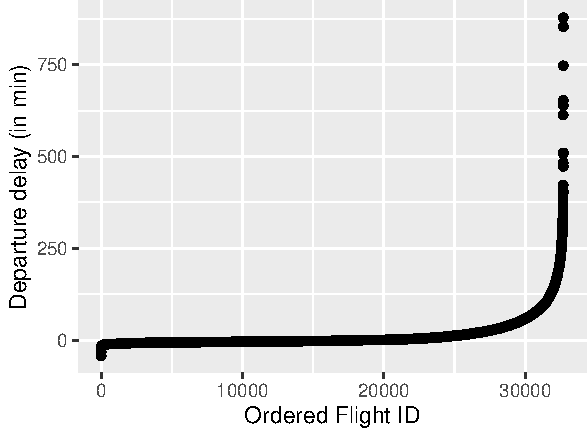
\includegraphics{Human-Centered-Data-Viz_files/figure-latex/chunk-label4-1.pdf}
\caption{\label{fig:chunk-label4}Second scatterplot of delay times.}
\end{figure}

What do you think of this chart? What can you say about flight delay times now? In the following, we focus on the delays only, since many flights seems to be one time.

\begin{Shaded}
\begin{Highlighting}[]
\CommentTok{\# dimensions of the data set}
\FunctionTok{dim}\NormalTok{(fly.sample)}
\end{Highlighting}
\end{Shaded}

\begin{verbatim}
## [1] 32674    19
\end{verbatim}

\begin{Shaded}
\begin{Highlighting}[]
\CommentTok{\# Remove all flights with no delay}
\NormalTok{fly.sample }\OtherTok{\textless{}{-}} \FunctionTok{subset}\NormalTok{(fly.sample, dep\_delay}\SpecialCharTok{\textgreater{}}\DecValTok{0}\NormalTok{)}

\CommentTok{\# dimensions of the data set}
\FunctionTok{dim}\NormalTok{(fly.sample)}
\end{Highlighting}
\end{Shaded}

\begin{verbatim}
## [1] 12843    19
\end{verbatim}

\hypertarget{histogram}{%
\subsection{Histogram}\label{histogram}}

Let's now create a graphical summary of these variables. Let's start with a histogram. It divides the range of the dep\_delay attribute into equal-sized bins and then plots the number of observations within each bin. What additional information does this new visualization give us about this variable?

The idiom of histograms shows the distribution of elements within an attribute. In the example, you can see a histogram of the weight distribution for all cats in a neighborhood, binned into 5-pound ranges.

The visual coding of a histogram is very similar to bar charts, with a line marker. One difference is that histograms are sometimes displayed with no space between bars to visually imply continuity, while bar charts conversely have spaces between bars to imply discretization. Despite their visual similarity, histograms are very different from bar charts. They do not show the original data but aggregate it.

The number of bins in the histogram can be chosen independently of the number of elements in the data set. The choice of bin size is crucial and tricky: a histogram can look very different depending on the discretization chosen. One possible solution to the problem is to calculate the number of bins based on the features of the data set; another is to provide controls for the user to interactively change the number of bins and see how the histogram changes.

\begin{longtable}[]{@{}
  >{\raggedright\arraybackslash}p{(\columnwidth - 2\tabcolsep) * \real{0.35}}
  >{\raggedright\arraybackslash}p{(\columnwidth - 2\tabcolsep) * \real{0.65}}@{}}
\caption{Characteristics of a histogram \citep{munzner2014visualization}}\tabularnewline
\toprule
Idiom & Histogram \\
\midrule
\endfirsthead
\toprule
Idiom & Histogram \\
\midrule
\endhead
What: Data & Table: one quantitative value attribute. \\
What: Derived & Derived table: one derived ordered key attribute (bin), one derived quantitative value attribute (item count per bin). \\
How: Encode & Rectilinear Layout. Line mark with aligned position to express derived value attribute. Position: key attribute. \\
\bottomrule
\end{longtable}

\begin{Shaded}
\begin{Highlighting}[]
\CommentTok{\# Visualize Data {-} Histogram}
\FunctionTok{ggplot}\NormalTok{(fly.sample, }\FunctionTok{aes}\NormalTok{(}\AttributeTok{x=}\NormalTok{dep\_delay)) }\SpecialCharTok{+} \FunctionTok{geom\_histogram}\NormalTok{() }\SpecialCharTok{+}
  \FunctionTok{xlab}\NormalTok{(}\StringTok{"Departure delay (in min)"}\NormalTok{) }\SpecialCharTok{+} \FunctionTok{ylab}\NormalTok{(}\StringTok{"Number of Flights"}\NormalTok{)  }
\end{Highlighting}
\end{Shaded}

\begin{figure}
\centering
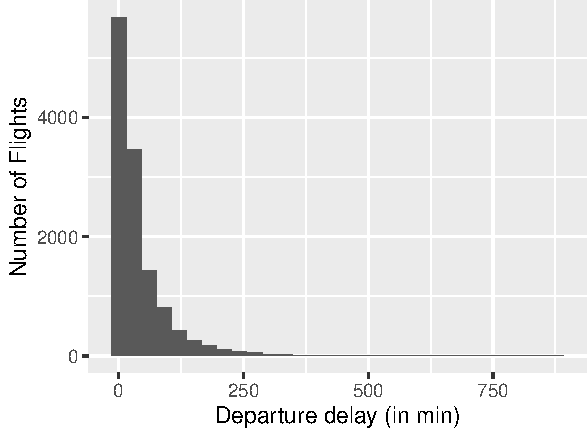
\includegraphics{Human-Centered-Data-Viz_files/figure-latex/chunk-label6-1.pdf}
\caption{\label{fig:chunk-label6}Histogram of Delay Times.}
\end{figure}

In the standard function the number of bins are 30, but of course, you can change them easily. The choice of binwidth significantly affects the resulting plot. Smaller binwidths can make the plot cluttered, but larger binwidths may obscure nuances in the data.

\begin{Shaded}
\begin{Highlighting}[]
\CommentTok{\#Change the size of the bins}
\FunctionTok{ggplot}\NormalTok{(fly.sample, }\FunctionTok{aes}\NormalTok{(}\AttributeTok{x=}\NormalTok{dep\_delay)) }\SpecialCharTok{+} \FunctionTok{geom\_histogram}\NormalTok{(}\AttributeTok{binwidth =} \DecValTok{1}\NormalTok{)  }\SpecialCharTok{+}
  \FunctionTok{xlab}\NormalTok{(}\StringTok{"Departure delay (in min)"}\NormalTok{) }\SpecialCharTok{+} \FunctionTok{ylab}\NormalTok{(}\StringTok{"Number of Flights"}\NormalTok{)}

\FunctionTok{ggplot}\NormalTok{(fly.sample, }\FunctionTok{aes}\NormalTok{(}\AttributeTok{x=}\NormalTok{dep\_delay)) }\SpecialCharTok{+} \FunctionTok{geom\_histogram}\NormalTok{(}\AttributeTok{binwidth =} \DecValTok{5}\NormalTok{)  }\SpecialCharTok{+}
  \FunctionTok{xlab}\NormalTok{(}\StringTok{"Departure delay (in min)"}\NormalTok{) }\SpecialCharTok{+} \FunctionTok{ylab}\NormalTok{(}\StringTok{"Number of Flights"}\NormalTok{)}

\FunctionTok{ggplot}\NormalTok{(fly.sample, }\FunctionTok{aes}\NormalTok{(}\AttributeTok{x=}\NormalTok{dep\_delay)) }\SpecialCharTok{+} \FunctionTok{geom\_histogram}\NormalTok{(}\AttributeTok{binwidth =} \DecValTok{10}\NormalTok{) }\SpecialCharTok{+}
  \FunctionTok{xlab}\NormalTok{(}\StringTok{"Departure delay (in min)"}\NormalTok{) }\SpecialCharTok{+} \FunctionTok{ylab}\NormalTok{(}\StringTok{"Number of Flights"}\NormalTok{)}

\FunctionTok{ggplot}\NormalTok{(fly.sample, }\FunctionTok{aes}\NormalTok{(}\AttributeTok{x=}\NormalTok{dep\_delay)) }\SpecialCharTok{+} \FunctionTok{geom\_histogram}\NormalTok{(}\AttributeTok{binwidth =} \DecValTok{15}\NormalTok{) }\SpecialCharTok{+}
  \FunctionTok{xlab}\NormalTok{(}\StringTok{"Departure delay (in min)"}\NormalTok{) }\SpecialCharTok{+} \FunctionTok{ylab}\NormalTok{(}\StringTok{"Number of Flights"}\NormalTok{)}
\end{Highlighting}
\end{Shaded}

\begin{figure}

{\centering \subfloat[(a)\label{fig:chunk-label7-1}]{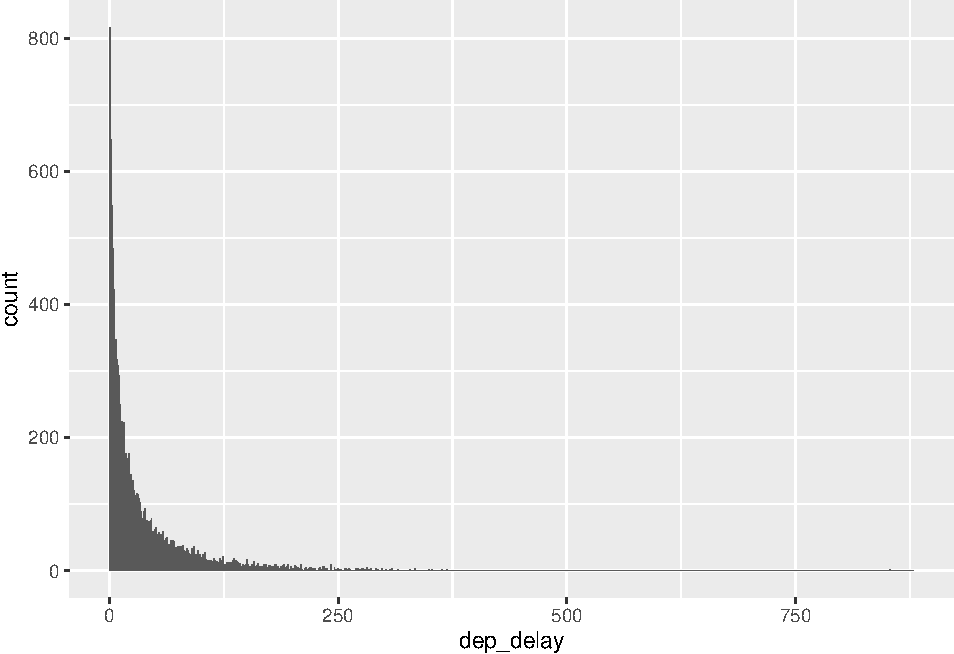
\includegraphics[width=0.5\linewidth]{Human-Centered-Data-Viz_files/figure-latex/chunk-label7-1} }\subfloat[(b)\label{fig:chunk-label7-2}]{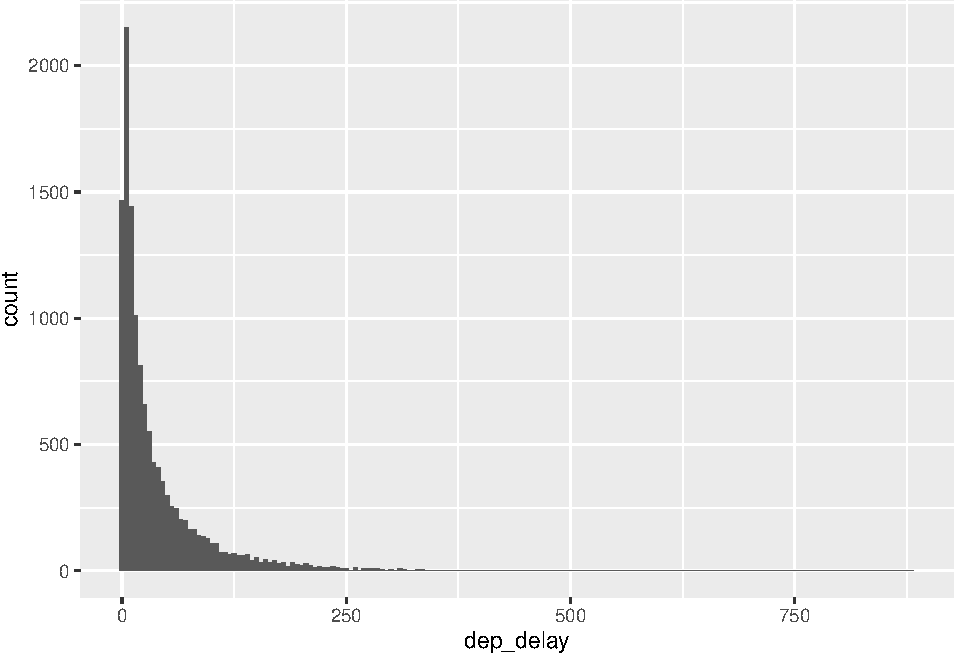
\includegraphics[width=0.5\linewidth]{Human-Centered-Data-Viz_files/figure-latex/chunk-label7-2} }\newline\subfloat[(c)\label{fig:chunk-label7-3}]{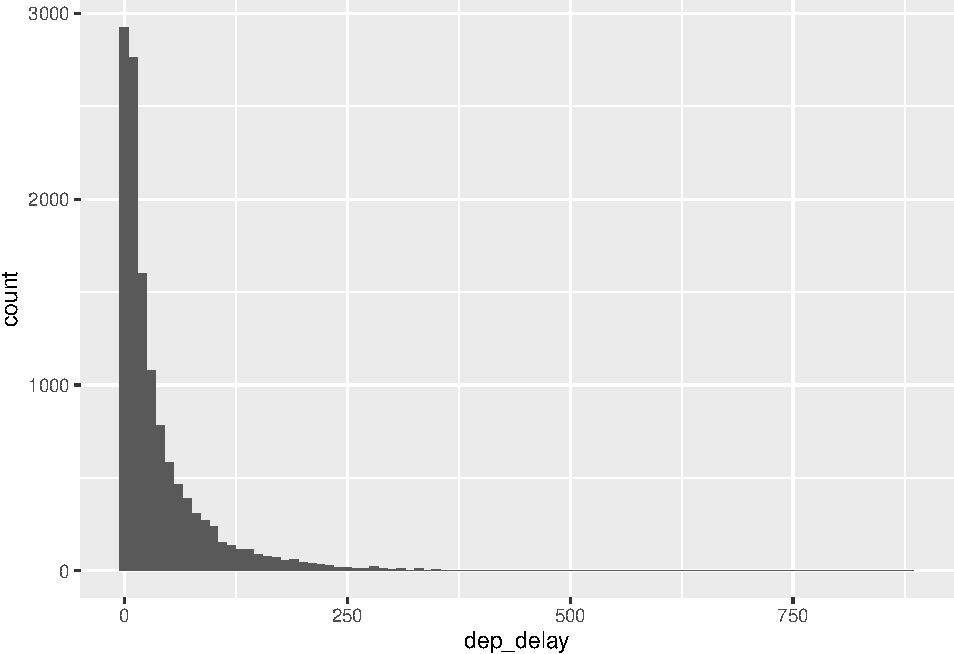
\includegraphics[width=0.5\linewidth]{Human-Centered-Data-Viz_files/figure-latex/chunk-label7-3} }\subfloat[(d)\label{fig:chunk-label7-4}]{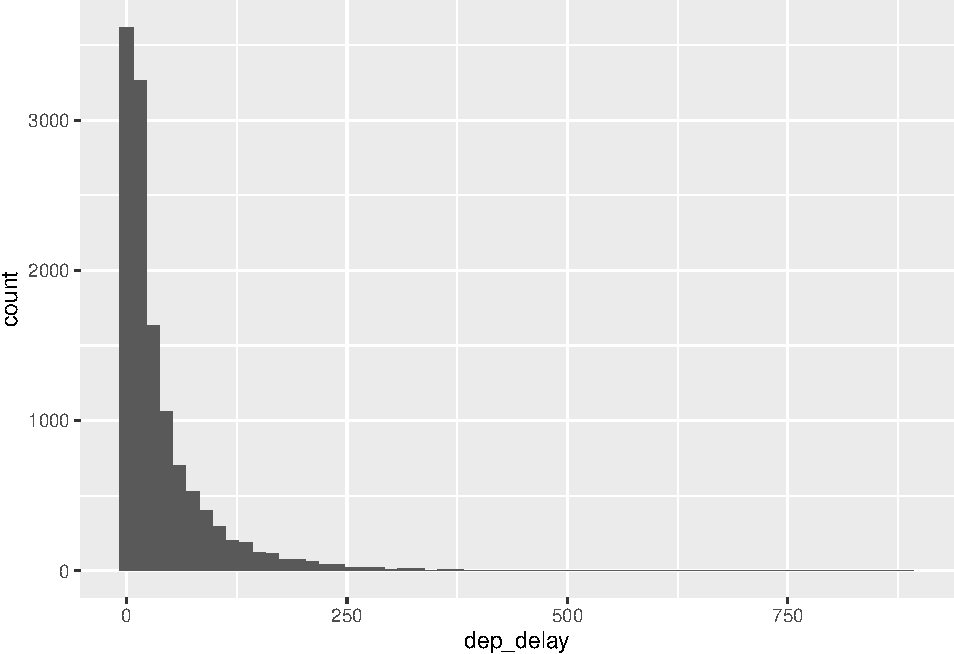
\includegraphics[width=0.5\linewidth]{Human-Centered-Data-Viz_files/figure-latex/chunk-label7-4} }

}

\caption{Histogram of Delay Times.}\label{fig:chunk-label7}
\end{figure}

\hypertarget{density-plot}{%
\subsection{Density Plot}\label{density-plot}}

A Density Plot is a smoothed, continuous version of a histogram that visualizes the underlying probability distribution of the data by a continuous curve\footnote{An excellent introduction in the usefulness of this method is given by Claus Wilke, check out \url{https://clauswilke.com/dataviz/histograms-density-plots.html}}. The peaks of a Density Plot help display where values are concentrated over the interval. The most common form of estimation is known as \href{https://en.wikipedia.org/wiki/Kernel_density_estimation}{kernel density estimation}. In this method, a continuous curve (the kernel) is drawn at every individual data point and all of these curves are then added together to make a single smooth density estimation. The kernel most often used is a Gaussian (which produces a Gaussian bell curve at each data point).

Just as is in the case with histograms, the exact visual appearance of a density plot depends on the kernel and bandwidth choices. In addition, the choice of the kernel affects the shape of the density curve.

\begin{Shaded}
\begin{Highlighting}[]
\CommentTok{\# Visualize Data {-} Density Plot}
\FunctionTok{ggplot}\NormalTok{(fly.viz2, }\FunctionTok{aes}\NormalTok{(}\AttributeTok{x=}\NormalTok{dep\_delay)) }\SpecialCharTok{+} 
  \FunctionTok{geom\_density}\NormalTok{(}\AttributeTok{color=}\StringTok{"darkblue"}\NormalTok{, }\AttributeTok{fill=}\StringTok{"lightblue"}\NormalTok{)  }\SpecialCharTok{+}
  \FunctionTok{xlab}\NormalTok{(}\StringTok{"Departure delay (in min)"}\NormalTok{)}
\end{Highlighting}
\end{Shaded}

\begin{figure}
\centering
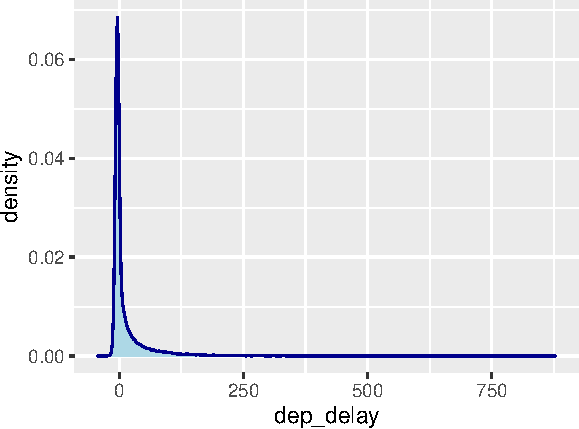
\includegraphics{Human-Centered-Data-Viz_files/figure-latex/chunk-label8-1.pdf}
\caption{\label{fig:chunk-label8}Density Plot of Delay Times.}
\end{figure}

\hypertarget{boxplot}{%
\subsection{Boxplot}\label{boxplot}}

Another alternative to display the distribution of a continuous variable broken down by a categorical variable is the Boxplot. The boxplot is an idiom presenting summary statistics for the distribution of a quantitative attribute, using five derived values (cp.~Figure ??).

\begin{figure}

{\centering 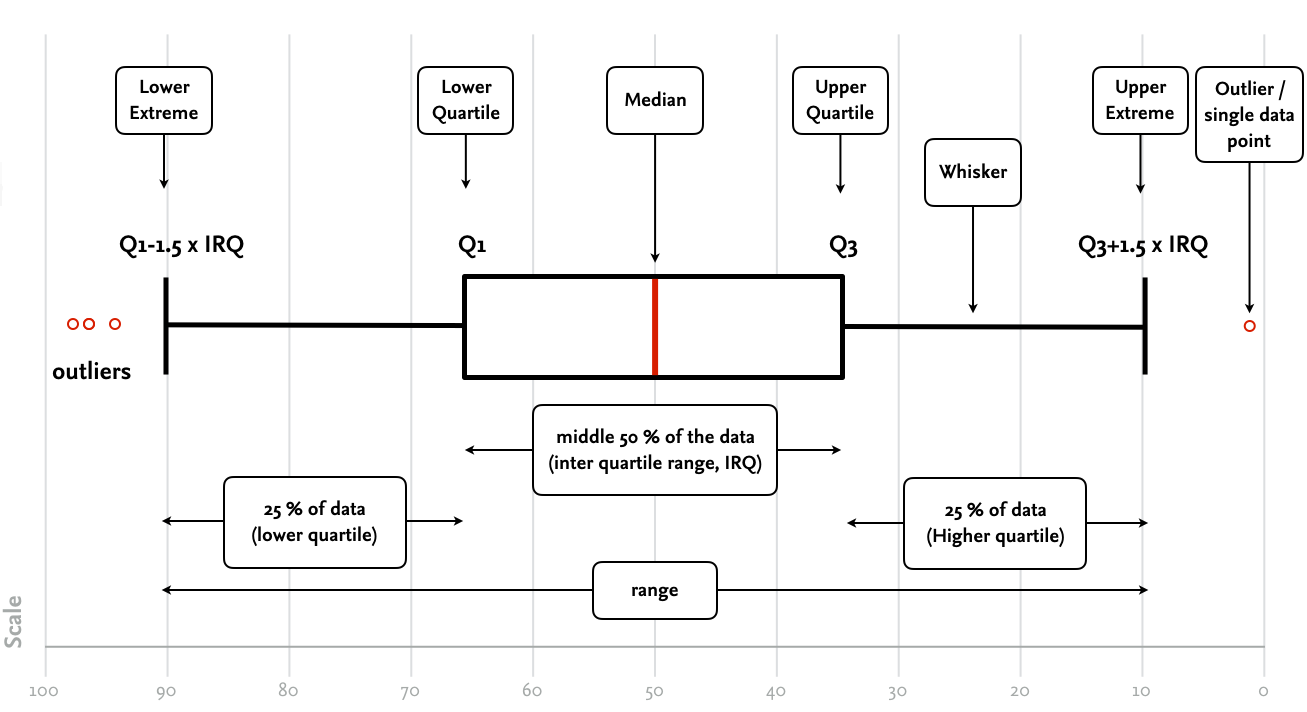
\includegraphics[width=1\linewidth]{images/boxplot} 

}

\caption{Properties of a Boxplot}\label{fig:unnamed-chunk-7}
\end{figure}

A box that extends from the \emph{25th percentile} (lower quartile, Q1) of the distribution to the \emph{75th percentile} (higher quartile, Q3), a distance called the \emph{interquartile range} (IQR). In the center of the box is a line indicating the \emph{median}, or 50th percentile, of the distribution. These three lines give you an idea of the spread of the distribution and whether the distribution is symmetrical about the median or skewed to one side. Furthermore, a line (or whisker) extending from each end of the box to the furthest non-outlier point (Q1-1.5 x IRQ and Q3+1.5 x IRQ) in the distribution which indicates the \emph{range}. Visual points indicating observations that fall more than 1.5 times the IQR from each edge of the box. These outer points are unusual, so they are plotted individually.

Boxplots are useful when we want to visualize many distributions at once and/or if we are primarily interested in overall shifts among the distributions.

\begin{longtable}[]{@{}
  >{\raggedright\arraybackslash}p{(\columnwidth - 2\tabcolsep) * \real{0.26}}
  >{\raggedright\arraybackslash}p{(\columnwidth - 2\tabcolsep) * \real{0.74}}@{}}
\caption{Characteristics of a boxplot \citep{munzner2014visualization}}\tabularnewline
\toprule
Idiom & Boxplot \\
\midrule
\endfirsthead
\toprule
Idiom & Boxplot \\
\midrule
\endhead
What: Data & Table: many quantitative value attributes. \\
What:Derived & Five quantitative attributes for each original attribute, representing its distribution. \\
Why: Task & Characterize distribution; find others, extremes, averages; identify skew. \\
How: Encode & One glyph per original attribute expressing derived attribute values using vertical spatial position, with 1D list alignment of glyphs into separated with horizontal spatial position. \\
How: Reduce & Item aggregation. \\
Scale & Items: unlimited. Attributes: dozens. \\
\bottomrule
\end{longtable}

\begin{Shaded}
\begin{Highlighting}[]
\CommentTok{\# Visualize Data {-} Box Plot }
\FunctionTok{ggplot}\NormalTok{(fly.viz2, }\FunctionTok{aes}\NormalTok{(}\AttributeTok{x=}\StringTok{\textquotesingle{}\textquotesingle{}}\NormalTok{,}\AttributeTok{y=}\NormalTok{dep\_delay)) }\SpecialCharTok{+} \FunctionTok{geom\_boxplot}\NormalTok{()}
\end{Highlighting}
\end{Shaded}

\begin{figure}
\centering
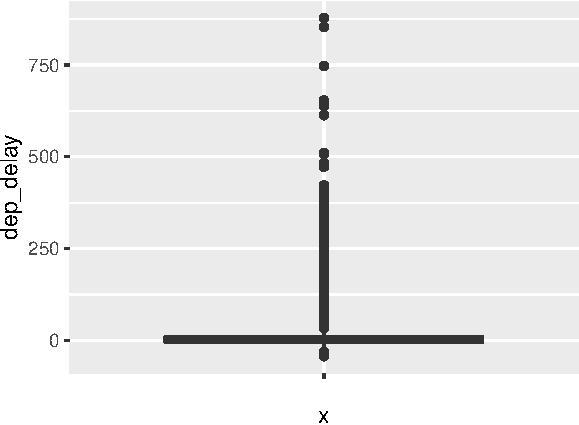
\includegraphics{Human-Centered-Data-Viz_files/figure-latex/chunk-label9-1.pdf}
\caption{\label{fig:chunk-label9}Boxplot of Delay Times.}
\end{figure}

\begin{Shaded}
\begin{Highlighting}[]
\CommentTok{\# the function mutate() adds new variables and preserves existing ones}
\NormalTok{fly.viz2 }\OtherTok{\textless{}{-}} \FunctionTok{mutate}\NormalTok{(fly.viz2, }\AttributeTok{min\_delay=}\FunctionTok{min}\NormalTok{(fly.viz2}\SpecialCharTok{$}\NormalTok{dep\_delay, }\AttributeTok{na.rm=}\ConstantTok{TRUE}\NormalTok{)) }
\NormalTok{fly.viz2 }\OtherTok{\textless{}{-}} \FunctionTok{mutate}\NormalTok{(fly.viz2, }\AttributeTok{log\_dep\_delay =} \FunctionTok{log}\NormalTok{(fly.viz2}\SpecialCharTok{$}\NormalTok{dep\_delay }\SpecialCharTok{{-}}\NormalTok{ fly.viz2}\SpecialCharTok{$}\NormalTok{min\_delay)) }

\CommentTok{\# Visualize Data {-} Box Plot with log scale}
\FunctionTok{ggplot}\NormalTok{(fly.viz2, }\FunctionTok{aes}\NormalTok{(}\AttributeTok{x=}\StringTok{\textquotesingle{}\textquotesingle{}}\NormalTok{, }\AttributeTok{y=}\NormalTok{log\_dep\_delay)) }\SpecialCharTok{+} \FunctionTok{geom\_boxplot}\NormalTok{()}
\end{Highlighting}
\end{Shaded}

\begin{figure}
\centering
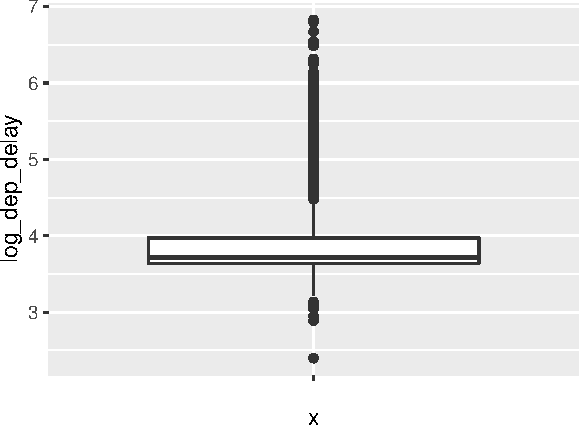
\includegraphics{Human-Centered-Data-Viz_files/figure-latex/chunk-label10-1.pdf}
\caption{\label{fig:chunk-label10}Boxplot of Delay Times (log scale).}
\end{figure}

\hypertarget{compare-distributions}{%
\subsection{Compare Distributions}\label{compare-distributions}}

Now we can start looking at the relationship between pairs of attributes. That is, how are each of the distributional properties we care about (central trend, spread and skew) of the values of an attribute changing based on the value of a different attribute. Suppose we want to see the relationship between departure delay time (a numeric variable), and the airport origin (a categorical variable).

\begin{Shaded}
\begin{Highlighting}[]
\CommentTok{\# Visualize Data {-} Box Plot in groups}
\FunctionTok{ggplot}\NormalTok{(fly.viz2, }\FunctionTok{aes}\NormalTok{(}\AttributeTok{x=}\NormalTok{origin, }\AttributeTok{y=}\NormalTok{log\_dep\_delay)) }\SpecialCharTok{+} \FunctionTok{geom\_boxplot}\NormalTok{() }\SpecialCharTok{+}
  \FunctionTok{ylab}\NormalTok{(}\StringTok{"Delay Times (in min)"}\NormalTok{)}
\end{Highlighting}
\end{Shaded}

\begin{figure}
\centering
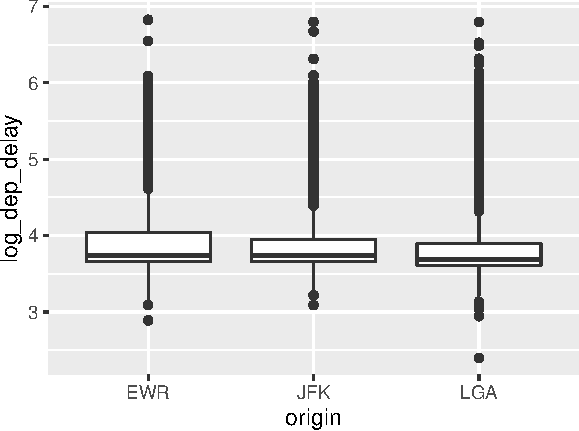
\includegraphics{Human-Centered-Data-Viz_files/figure-latex/chunk-label11-1.pdf}
\caption{\label{fig:chunk-label11}Multiple Boxplots of Delay Times depending on airport origine.}
\end{figure}

\hypertarget{summary-statistics}{%
\subsection{Summary Statistics}\label{summary-statistics}}

Let's continue our discussion of exploratory data analysis. In the previous section, we saw ways to visualize attributes (variables) using graphs to begin understanding the properties of the data distribution, an essential and preliminary step in data analysis. In this section, we begin discussing statistical or numerical summaries of data to quantify properties we have observed using visual summaries and plots. Remember that one purpose of EDA is to identify problems in data and understand variable properties. We also want to use EDA to understand the relationship between pairs of variables, such as their correlation or covariance.

We differentiate measures of central tendency, i.e., measures of location that describe a tendency of data to center about certain numerical value. Here we have mode, median, and mean. Then we have measures of variability, i.e., dispersion that describe the spread of the data across possible values. To this group the range, interquartile range, variance, and standard deviation belong to. Finally we have measures of shape that relate to the form of the distribution, its skewness.

In this chapter, we use the diamond data set, that contains the prices, carat, color and other attributes of almost 54,000 diamonds.

\begin{Shaded}
\begin{Highlighting}[]
\CommentTok{\#library(skimr)}

\CommentTok{\# load dataset and show structure}
\FunctionTok{data}\NormalTok{(diamonds)}
\CommentTok{\# skim(diamonds)}

\CommentTok{\# show attributes only}
\FunctionTok{names}\NormalTok{(diamonds)}
\end{Highlighting}
\end{Shaded}

\begin{verbatim}
##  [1] "carat"   "cut"     "color"   "clarity" "depth"   "table"   "price"  
##  [8] "x"       "y"       "z"
\end{verbatim}

\begin{Shaded}
\begin{Highlighting}[]
\CommentTok{\# count frequencies}
\FunctionTok{table}\NormalTok{(diamonds}\SpecialCharTok{$}\NormalTok{cut)}
\end{Highlighting}
\end{Shaded}

\begin{verbatim}
## 
##      Fair      Good Very Good   Premium     Ideal 
##      1610      4906     12082     13791     21551
\end{verbatim}

\begin{Shaded}
\begin{Highlighting}[]
\CommentTok{\# counts proportions}
\FunctionTok{prop.table}\NormalTok{(}\FunctionTok{table}\NormalTok{(diamonds}\SpecialCharTok{$}\NormalTok{cut))}
\end{Highlighting}
\end{Shaded}

\begin{verbatim}
## 
##       Fair       Good  Very Good    Premium      Ideal 
## 0.02984798 0.09095291 0.22398962 0.25567297 0.39953652
\end{verbatim}

Part of our goal is to understand how the variables are distributed in a given data set. Again, note that we are not using distribution in a formal mathematical (or probabilistic) sense. All the statements we make here are based on the data at hand, so we might call this an empirical distribution of data. Empirical is used here in the sense that it is data resulting from an experiment. Let's take a data set on the properties of diamonds as an example.

\begin{Shaded}
\begin{Highlighting}[]
\CommentTok{\# dimensions of the data set}
\FunctionTok{ggplot}\NormalTok{(diamonds, }\FunctionTok{aes}\NormalTok{(}\AttributeTok{x=}\NormalTok{depth)) }\SpecialCharTok{+} \FunctionTok{geom\_histogram}\NormalTok{(}\AttributeTok{bins=}\DecValTok{100}\NormalTok{)}
\end{Highlighting}
\end{Shaded}

\begin{figure}
\centering
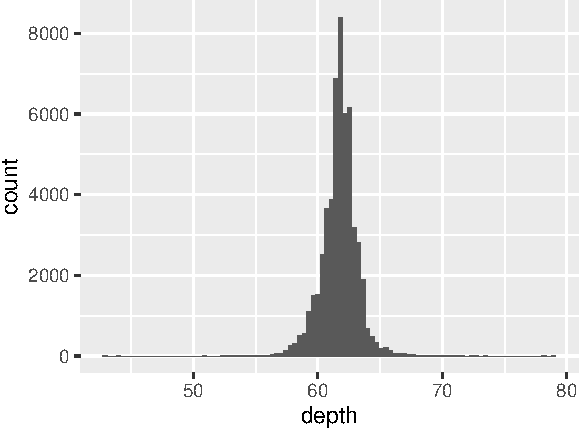
\includegraphics{Human-Centered-Data-Viz_files/figure-latex/chunk-label13-1.pdf}
\caption{\label{fig:chunk-label13}Distribution of Depth in the Diamonds Data Set.}
\end{figure}

\hypertarget{central-tendency}{%
\subsection{Central Tendency}\label{central-tendency}}

Now that we know the area over which the data is distributed, we can figure out an initial summary of the data over that area. Let's start with the center of the data:

The median is a statistic defined such that half of the data has a smaller value. We can use the notation \texttt{x(n/2)} (a rank statistic) to represent the median.

Note that we can use an algorithm based on the quicksort partition scheme to compute the median in linear time (on average).

\(\bar{x} = \frac{1}{n}\sum_{i=1}^{n} x_{i}\).

Where is the mean in our example dataset?

\begin{Shaded}
\begin{Highlighting}[]
\CommentTok{\# determine median}
\FunctionTok{ggplot}\NormalTok{(diamonds, }\FunctionTok{aes}\NormalTok{(}\AttributeTok{x=}\NormalTok{depth)) }\SpecialCharTok{+} \FunctionTok{geom\_histogram}\NormalTok{(}\AttributeTok{bins=}\DecValTok{100}\NormalTok{) }\SpecialCharTok{+} \FunctionTok{geom\_vline}\NormalTok{(}\FunctionTok{aes}\NormalTok{(}\AttributeTok{xintercept=}\FunctionTok{median}\NormalTok{(depth)), }\AttributeTok{color=}\StringTok{"red"}\NormalTok{)}
\end{Highlighting}
\end{Shaded}

\begin{figure}
\centering
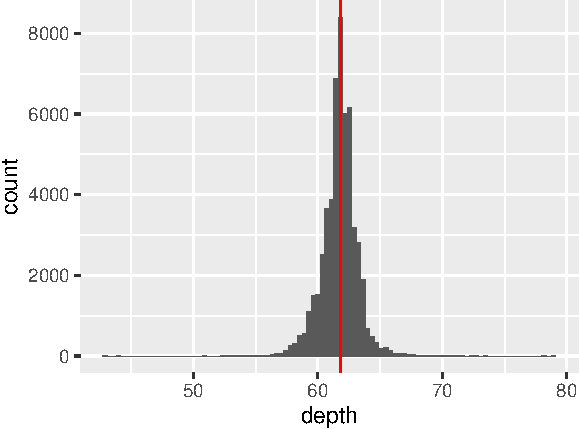
\includegraphics{Human-Centered-Data-Viz_files/figure-latex/chunk-label14-1.pdf}
\caption{\label{fig:chunk-label14}Show Mean in Distribution of Depth in the Diamonds Data Set.}
\end{figure}

Now that we have a measure of the center, we can now discuss how the data is distributed around that center.

\hypertarget{median-and-iqr}{%
\subsection{Median, and IQR}\label{median-and-iqr}}

Median is better measure of central tendency than the mean when we have outliers or/and skewed distribution, e.g., income, housing prices, waiting time. It is the middle observation when data is sorted in the order of magnitude. Thus (about) 50 \% of observations are smaller and (about) 50 \% are larger than the median. In our dataset:

\begin{Shaded}
\begin{Highlighting}[]
\CommentTok{\# min and max value}
\FunctionTok{summarize}\NormalTok{(diamonds, }\AttributeTok{min\_depth =} \FunctionTok{min}\NormalTok{(diamonds}\SpecialCharTok{$}\NormalTok{depth), }\AttributeTok{max\_depth =} \FunctionTok{max}\NormalTok{(diamonds}\SpecialCharTok{$}\NormalTok{depth))}
\end{Highlighting}
\end{Shaded}

\begin{verbatim}
## # A tibble: 1 x 2
##   min_depth max_depth
##       <dbl>     <dbl>
## 1        43        79
\end{verbatim}

\begin{Shaded}
\begin{Highlighting}[]
\CommentTok{\# mean vs. median}
\FunctionTok{summarize}\NormalTok{(diamonds, }\AttributeTok{mean\_depth =} \FunctionTok{mean}\NormalTok{(diamonds}\SpecialCharTok{$}\NormalTok{depth), }\AttributeTok{median\_depth =} \FunctionTok{median}\NormalTok{(diamonds}\SpecialCharTok{$}\NormalTok{depth))}
\end{Highlighting}
\end{Shaded}

\begin{verbatim}
## # A tibble: 1 x 2
##   mean_depth median_depth
##        <dbl>        <dbl>
## 1       61.7         61.8
\end{verbatim}

For the mean, we have a convenient way to describe this: the average distance (using the squared difference) from the mean. We call this the variance of the data. vhe Variance is a commonly used statistic for dispersion, but it has the disadvantage that its units are not easily conceptualized (e.g., squared diamond depth).

\(sd(x) = \frac{1}{n} \sum_{i-1}^n (x_i-\bar{x})^2\)

A scatter statistic that is in the same units as the data is the standard deviation, which is just the square root of the variance:

\(var(x) = \sqrt{\frac{1}{n} \sum_{i-1}^n (x_i-\bar{x})^2}\)

We can also use standard deviations as an interpretable unit for how far a particular data point is from the mean. This is often use in tables.

Just like we saw how the median is a rank statistic used to describe central tendency, we can also use rank statistics to describe spread.
For this we use two more rank statistics: the first and third quartiles, x(n/4) and x(3n/4) respectively. We know this already, it is the interquartile range. Also called midspread and is the difference between third and first quartiles (spread in the middle 50\%).
It is not affected by extreme values.

\begin{Shaded}
\begin{Highlighting}[]
\CommentTok{\# Rang}
\FunctionTok{range}\NormalTok{(diamonds}\SpecialCharTok{$}\NormalTok{depth)}
\end{Highlighting}
\end{Shaded}

\begin{verbatim}
## [1] 43 79
\end{verbatim}

\begin{Shaded}
\begin{Highlighting}[]
\CommentTok{\# Variance}
\FunctionTok{var}\NormalTok{(diamonds}\SpecialCharTok{$}\NormalTok{depth)}
\end{Highlighting}
\end{Shaded}

\begin{verbatim}
## [1] 2.052404
\end{verbatim}

\begin{Shaded}
\begin{Highlighting}[]
\CommentTok{\#standard deviation}
\FunctionTok{sd}\NormalTok{(diamonds}\SpecialCharTok{$}\NormalTok{depth)}
\end{Highlighting}
\end{Shaded}

\begin{verbatim}
## [1] 1.432621
\end{verbatim}

\hypertarget{outliers}{%
\subsection{Outliers}\label{outliers}}

There is no precise way to define and identify outliers. Instead, a subject matter expert must interpret the raw observations and decide whether or not a value is an outlier.

\begin{Shaded}
\begin{Highlighting}[]
\FunctionTok{library}\NormalTok{(outliers)}

\CommentTok{\# Determine outlier (Finds value with largest difference between it and sample mean, which can be an outlier.)}
\FunctionTok{outlier}\NormalTok{(diamonds}\SpecialCharTok{$}\NormalTok{depth)}
\end{Highlighting}
\end{Shaded}

\begin{verbatim}
## [1] 43
\end{verbatim}

However, we can use estimates of dispersion to identify outlier values in a data set. If we make an estimate of dispersion based on the techniques we have just seen, we can identify values that are unusually far from the center of the distribution. Although this method works relatively well in practice, it presents a fundamental problem. Severe outliers can significantly affect standard deviation-based spread estimates. In particular, the spread estimates are inflated in the presence of severe outliers. To circumvent this problem, we use rank-based spread estimates to identify outliers as such:
\(outliers_{sd}(x)= \{x_i||x_j|>\bar{x}+k \times sd(x)\}\)

To mitigate the effect of severe outliers you can use rank-based estimates of spread to identify outliers as:

\(\mbox{outliers}_{IQR}(x)= \{x_j|x_j < x_{(1/4)} - k \times IQR(x) \mbox{ or } x_j > x_{(3/4)} + k \times IQR(x) \}\)

This is usually referred to as the Tukey outlier rule, where the multiplier k plays the same role as before. We use IQR here because it is less prone to inflating due to severe outliers in the data set. It also works better for skewed data than the standard deviation based method.

\begin{figure}
\centering
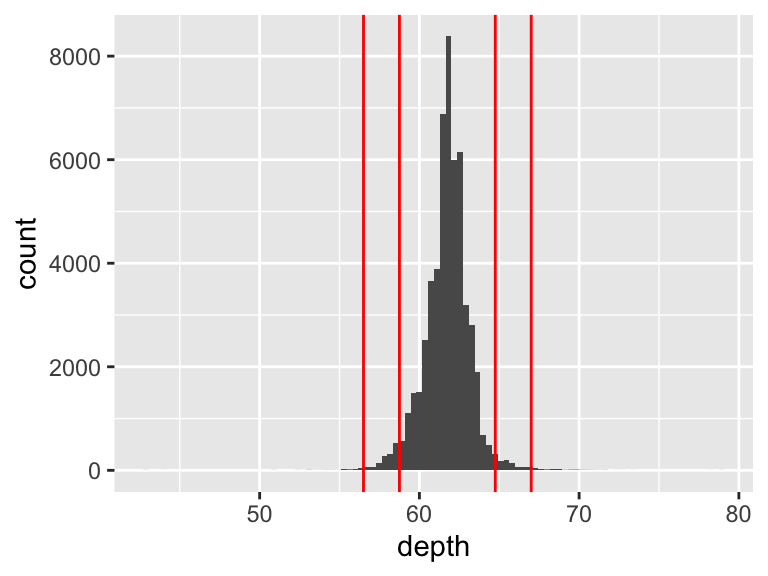
\includegraphics{Human-Centered-Data-Viz_files/figure-latex/chunk-label17a-1.pdf}
\caption{\label{fig:chunk-label17a}Spread of Depth in the Diamonds Data Set.}
\end{figure}

When does it make sense to remove outliers?

Well, it depends. As you can see in this visualization, removing outliers can distort your analyses by removing important information from the dataset. However, you have to make an informed decision what to do with them because removing outliers is legitimate only for specific reasons. Outliers can provide very interesting information about the subject-area and data collection process. It's essential to understand how outliers occur and whether they might happen again as a normal part of the process or study area. You might be tempted to simply remove outliers to decrease the variability in your data and therefore the increases statistical power, which makes your results to become statistically significant. These temptation might be a reason for the reproducibility crisis in psychology and other disciplines.

\hypertarget{skewness}{%
\subsection{Skewness}\label{skewness}}

One final thought. Although there are formal ways to define this precisely, the five-number summary can be used to understand if data are biased. How?

If one of these differences is larger than the other, then it suggests that this data set may be skewed, meaning that the range of data on one side of the median is longer (or shorter) than the range of data on the other side of the median. Do you think our diamond depth data set is biased?

\begin{Shaded}
\begin{Highlighting}[]
\FunctionTok{library}\NormalTok{(moments)}

\CommentTok{\# Summary statistics}
\FunctionTok{summary}\NormalTok{(diamonds}\SpecialCharTok{$}\NormalTok{depth)}
\end{Highlighting}
\end{Shaded}

\begin{verbatim}
##    Min. 1st Qu.  Median    Mean 3rd Qu.    Max. 
##   43.00   61.00   61.80   61.75   62.50   79.00
\end{verbatim}

\begin{Shaded}
\begin{Highlighting}[]
\CommentTok{\# Skewness}
\FunctionTok{skewness}\NormalTok{(diamonds}\SpecialCharTok{$}\NormalTok{depth)}
\end{Highlighting}
\end{Shaded}

\begin{verbatim}
## [1] -0.08229174
\end{verbatim}

The skewness of the data is negative, thus, we can conclude that the data are close to bell shape but slightly skewed to the left.

For pairs of continuous variables, the most useful visualization is the scatter plot. This gives an idea of how a variable varies (in terms of central trend, variance and skewness) depending on another variable. A scatter plot can be used to show relationship between \texttt{price} and \texttt{carrat}.

\begin{Shaded}
\begin{Highlighting}[]
\CommentTok{\# Visualize Data {-} Scatterplot}
\FunctionTok{ggplot}\NormalTok{(diamonds, }\FunctionTok{aes}\NormalTok{(}\AttributeTok{x=}\NormalTok{price, }\AttributeTok{y=}\NormalTok{carat)) }\SpecialCharTok{+} \FunctionTok{geom\_point}\NormalTok{()}
\end{Highlighting}
\end{Shaded}

\begin{figure}
\centering
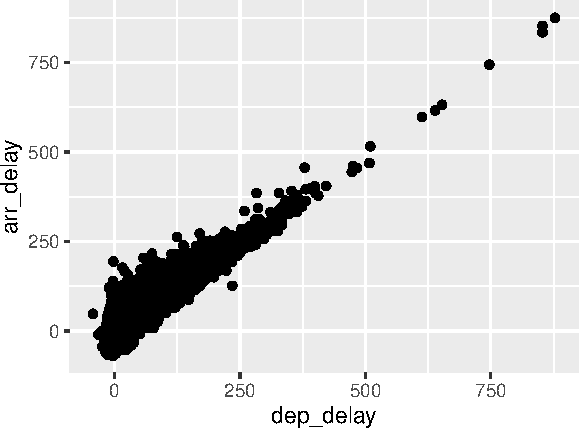
\includegraphics{Human-Centered-Data-Viz_files/figure-latex/chunk-label11-1-1.pdf}
\caption{\label{fig:chunk-label11-1}Scatterplot of Price Depending On Carat}
\end{figure}

As we expected, there seem to be a relationsship between price and carrat, which brings us to the next question.

\hypertarget{covariance-and-correlation}{%
\subsection{Covariance and Correlation}\label{covariance-and-correlation}}

As you have learned, the scatterplot is a visual method for observing relationships between pairs of variables.

\begin{Shaded}
\begin{Highlighting}[]
\CommentTok{\# Covariance and correlation}
\NormalTok{diamonds }\SpecialCharTok{\%\textgreater{}\%}
  \FunctionTok{ggplot}\NormalTok{(}\FunctionTok{aes}\NormalTok{(}\AttributeTok{x=}\NormalTok{carat, }\AttributeTok{y=}\NormalTok{price)) }\SpecialCharTok{+}
  \FunctionTok{geom\_point}\NormalTok{() }\SpecialCharTok{+}
  \FunctionTok{geom\_hline}\NormalTok{(}\FunctionTok{aes}\NormalTok{(}\AttributeTok{yintercept =} \FunctionTok{mean}\NormalTok{(price)), }\AttributeTok{color=}\StringTok{"blue"}\NormalTok{, }\AttributeTok{lty=}\DecValTok{2}\NormalTok{) }\SpecialCharTok{+}
  \FunctionTok{geom\_vline}\NormalTok{(}\FunctionTok{aes}\NormalTok{(}\AttributeTok{xintercept =} \FunctionTok{mean}\NormalTok{(carat)), }\AttributeTok{color=}\StringTok{"blue"}\NormalTok{, }\AttributeTok{lty=}\DecValTok{2}\NormalTok{)}
\end{Highlighting}
\end{Shaded}

\begin{figure}
\centering
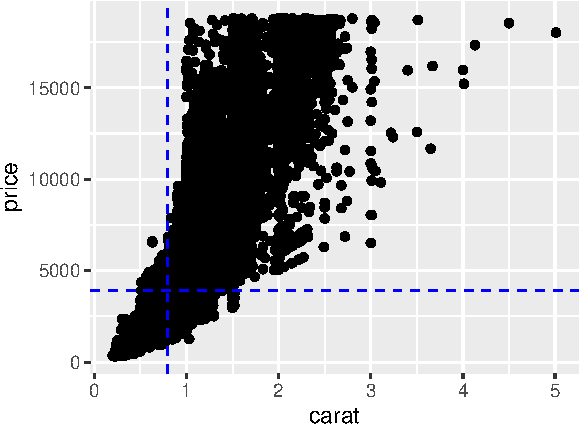
\includegraphics{Human-Centered-Data-Viz_files/figure-latex/chunk-label19-1.pdf}
\caption{\label{fig:chunk-label19}Covariance and correlation.}
\end{figure}

However, how do we quantitatively summarize the relationship between two variables. We need to extend our notion of scatter (or variation of data around the mean) to the notion of covariation: do pairs of variables vary around the mean in the same way or more precisly, does x\textasciitilde i vary in the same direction and on the same scale away from its mean as y\textasciitilde i?

This leads to covariance:
\(cov(x,y) =\frac{1}{n}\sum_{i=1}^{n}(x_i - \bar{x})(y_i -\bar{y})\)

Correlation (formally, Pearson's correlation coefficient) summarizes the same relationship in a unit-less way:

\(cor(x,y)=\frac{cov(x,y)}{sd(x)sd(y)}\)

Correlation evaluates the direction as well as strength of a relationship between continuous variables. The correlation coefficient can range from -1 to +1, which signifies strong negative to strong positive relation between the variables.

You can think of the correlation as the covariance between x and y after transforming each to the unitless scale of z-scores. Just to recall, a z-score of a sample x is defined as the mean-centered, scale normalized observations: \(z_i(x)=\frac{x_i-\bar{x}}{sd(x)}\), thus \(r(x,y)=cov(z(x),z(y))\).

\hypertarget{correlation-matrix}{%
\subsection{Correlation Matrix}\label{correlation-matrix}}

The covariance is a simple summary of association between two variables, but it certainly may not capture the whole ``story'' when dealing with more than two variables. The most common summary of multivariate relation, is the covariance matrix, but we warn that only the simplest multivariate relations are fully summarized by this matrix.

\begin{Shaded}
\begin{Highlighting}[]
\CommentTok{\# Correlation Matrix (less meaningful example {-} just a showcase)}

\NormalTok{diamonds\_corr }\OtherTok{\textless{}{-}} \FunctionTok{cor}\NormalTok{(diamonds[,}\FunctionTok{c}\NormalTok{(}\DecValTok{1}\NormalTok{,}\DecValTok{5}\NormalTok{,}\DecValTok{6}\NormalTok{,}\DecValTok{7}\NormalTok{)])}

\CommentTok{\# Print mcor and round to 2 digits}
\FunctionTok{round}\NormalTok{(diamonds\_corr, }\AttributeTok{digits=}\DecValTok{2}\NormalTok{)}
\end{Highlighting}
\end{Shaded}

\begin{verbatim}
##       carat depth table price
## carat  1.00  0.03  0.18  0.92
## depth  0.03  1.00 -0.30 -0.01
## table  0.18 -0.30  1.00  0.13
## price  0.92 -0.01  0.13  1.00
\end{verbatim}

\begin{Shaded}
\begin{Highlighting}[]
\CommentTok{\# Load visualization from package}
\FunctionTok{library}\NormalTok{(corrplot)}
\FunctionTok{corrplot}\NormalTok{(diamonds\_corr)}
\end{Highlighting}
\end{Shaded}

\begin{figure}
\centering
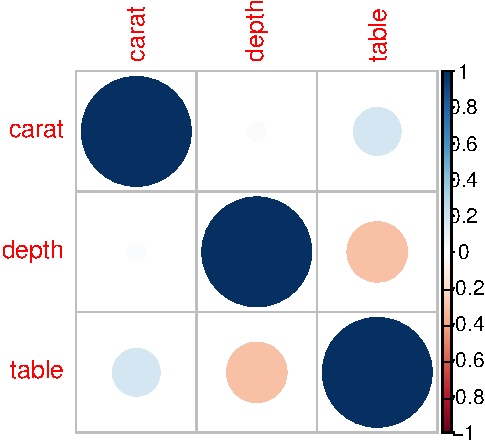
\includegraphics{Human-Centered-Data-Viz_files/figure-latex/chunk-label20-1.pdf}
\caption{\label{fig:chunk-label20}Correlation Matrix.}
\end{figure}

\hypertarget{general-guidelines-for-eda}{%
\section{General Guidelines for EDA}\label{general-guidelines-for-eda}}

It is difficult to say, what the best process is in EDA. I just provided a number of analyses and possible visualizations. You find many alternative suggestions, and I provide one of them:

\begin{itemize}
\tightlist
\item
  Begin with a discussion of the ``center'' of the data, generally based on mean.
\item
  Describes how data are distributed.
\item
  Follow with a discussion of variability (and of skew if appropriate).
\item
  End with a summary evaluation which may have a subjective component (numbers must be interpreted, they don't speak for themselves).
\item
  Make sure to use numbers in a description wisely -- not too few or too many.
\end{itemize}

However, each dataset is very special, thus, as often it stays to be an individualized process. Therefore, reproducibility is very important during EDA. Computational notebooks such as R Markdown (used here), but also Jupyter notebooks (used in our exercise), Observable (google product) support readability and understandability of your exploration process. This supports \href{https://en.wikipedia.org/wiki/Literate_programming}{Knuth's vision of literate programming}.

\hypertarget{tools-and-libraries-for-data-exploration}{%
\section{Tools and Libraries for Data Exploration}\label{tools-and-libraries-for-data-exploration}}

Besides GNY R there are many tools and libraries that support the process of data exploration. In this section, I provide a selection.

Wrangler provides data-transformation scripts within a visual, direct manipulation interface augmented by predictive models \citep{kandel2011wrangler}. Wrangler is an interactive system for creating data transformations. It uses semantic data types, such as geographic locations, dates, classification codes to support the validation of data and the type conversion. Interactive histories support review, refinement, and annotation of transformation scripts. The researchers provide a WebApp but also a \href{https://www.trifacta.com/start-wrangling/}{commercial product}.

A similar approach is realized by \href{https://openrefine.org/}{Open Refine}. This tool was formerly developed by Google but it is now maintained by the open source community. It allows you to clean data, transform it from one format into another, or extend you data by additional data from an API.

Besides DataWrangler, I would like to mention the tool Voyager \citep{wongsuphasawat2015voyager}. The Voyager system is specifically suitable for exploratory visual analysis. You can again test it via a \href{https://vega.github.io/voyager/}{WebApp} and the source code is available on \href{https://github.com/vega/voyager}{Github}. And for the sake of completeness, there is also a commercial software \href{https://www.tableau.com/}{Tableau}, which can be freely used in the educational context.

Both, Data Wrangler and Voyager are using a formal language - the Vega-Lite visualization grammar. Vega-Lite is a high-level grammar of interactive graphics that provides a concise, declarative JSON syntax to create diagrams for data analysis and presentation. Vega-Lite specifications describe visualizations as ``encoding mappings'\,' from data to properties of graphical marks (e.g., points or bars).

The Vega-Lite compiler automatically produces visualization components including axes, legends, and scales. Vega-Lite supports both data transformations (e.g., aggregation, binning, filtering, sorting) and visual transformations (e.g., stacking and faceting). Moreover, Vega-Lite specifications can be composed into layered and multi-view displays, and made interactive with selections as you can see in the example.

Vega-Lite is being used in another interesting library. On top of the Vega-Lite JSON specification a simple API was built: Altair. It is a declarative statistical visualization library for Python. \href{https://github.com/altair-viz/altair}{Source code} and a comprehensive \href{https://altair-viz.github.io/}{documentation} as well as \href{github.com/altair-viz/altair_notebooks}{Tutorial Notebooks} are available on Github.

\hypertarget{human-perception-and-visual-encoding}{%
\chapter{Human Perception and Visual Encoding}\label{human-perception-and-visual-encoding}}

As we have discussed on the previous chapters, an important first step in data visualization is to contextualize your data. The next step is to select - based on the data characteristics - an effective visual encoding. Such visual encoding maps the data values to graphical features such as position, size, shape, and color. However, such mapping is not as straightforward as one might assume. A prerequisite is to understand how we, as humans, perceive our world, or more specifically visualizations. Ware states in his book \citep{ware2019information}: `'Understanding human perception can significantly improve both the quality and the quantity of information being displayed.'' Such understanding allows us to design visualizations that can replace demanding cognitive calculations with simple perceptual inferences which often improve interpretability \& comprehension and, therefore, decision making \citep{Heer_Bostock_Ogievetsky_2010}.

\hypertarget{human-perception}{%
\section{Human Perception}\label{human-perception}}

Human perception is the ability to perceive our surroundings through the light that enters the eyes. The eye convert light into a series of electrochemical signals that are transmitted to the brain. This process can take as little as 13 milliseconds, according to a 2017 study by MIT in the United States \citep{munzner2014visualization}. However, human vision has a number of physical and perceptual limitations (concerning colors, patterns, and structures), which we should be aware of in order to create more effective data visualizations.

We can roughly divide perception into two stages \citep{Few2004showmenumbers}. The sensations is the physical reception of the stimulus from the outside world, and the perception is a cognitive process that relates to the processing and interpretation of that stimulus. On the one hand the physical properties of the eye and the visual system mean that there are certain things that cannot be seen by the human; on the other hand, the interpretative capabilities of visual processing allow images to be constructed from incomplete information.

We need to understand both stages as both influence what can and cannot be perceived visually by a human being, which in turn directly affects the way that we design visualizations.

We begin with looking at the eye as a physical receptor, and then go on to consider the processing involved in basic vision.

\hypertarget{the-human-eye}{%
\subsection{The Human Eye}\label{the-human-eye}}

Vision begins with light which is reflected from objects in the world. This light catches the eye and the image of these objects is projected upside down on the back of the eye, on the retina (this you might remember from school). In the following, we look into these components in more detail (cp.~Figure XX).

\begin{figure}

{\centering 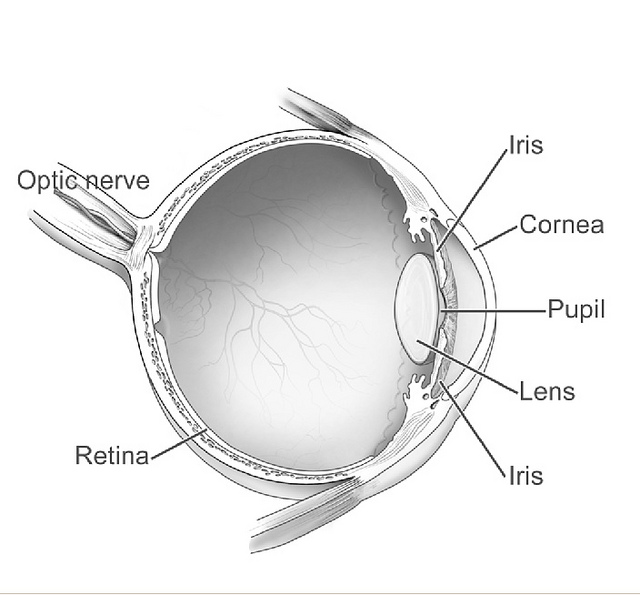
\includegraphics[width=0.5\linewidth]{images/humaneye} 

}

\caption{Components of the Human Eye, National Eye Institute. Taken from Wikipedia Commons}\label{fig:unnamed-chunk-8}
\end{figure}

At the front of the eye are the cornea and lens which focus the light into a sharp image on the retina. The retina is the the light-sensitive layer of the eye. In a person with normal vision, the lens focuses images perfectly on a small depression in the back of the eye called the fovea (in German Sehgrube), which is part of the retina.

The retina contains two types of photoreceptor (light-sensitive cells): rods for low-light vision and cones for color vision.

Rods are highly sensitive to light and therefore allow us to see under a low level of lightning. However, they are unable to resolve fine detail and are subject to light saturation. This is the reason for the temporary blindness we get when moving from a darkened room into sunlight: the rods have been active and are saturated by the sudden light. As you can imagine, nowadays in our industrialized world, rods are hardly used \citep{Johnson2014designingwiththemind}. There are approximately 120 million rods per eye which are mainly situated towards the edges of the retina. Rods therefore dominate peripheral vision.

The cones are specialized types of photoreceptors that work best in bright light conditions. Cones are very sensitive to acute detail and provide tremendous spatial resolution. They are also directly involved in our ability to perceive color. The eye has approximately 6 million cones, mainly concentrated on the fovea. We can differentiate three types of cones. Each type of cone is sensitive to a range of light frequencies, and these sensitivity ranges overlap considerably \citep{Johnson2014designingwiththemind}.

Although the retina is mainly covered with photoreceptors there is one blind spot where the optic nerve enters the eye. The blind spot has no rods or cones, yet our visual system compensates for this so that in normal circumstances we are unaware of it.

The retina also has specialized nerve cells called ganglion cells. There are two types: X-cells, which are concentrated in the fovea and are responsible for the early detection of pattern; and Y-cells which are more widely distributed in the retina and are responsible for the early detection of movement. The distribution of these cells means that, while we may not be able to detect changes in pattern in peripheral vision, we can perceive movement.

\hypertarget{color-vision}{%
\subsection{Color Vision}\label{color-vision}}

We can describe color by different color space presentation. The RGB is the most popular one. However, in 1970, computer graphics researchers developed a model that closely aligns with the way human vision perceives color: the HSL (for hue, saturation, lightness) model. Hue is described in units of degree starting from 0 (red) to 360º.These are the typical colors you know. Saturation measures the degree to which a particular hue fully exhibits its essence. It goes from 0 \% (grey) to 100\% (very colorful). Lightness (or brightness) measures the degree to which color appears dark or light ranging from 0\% (black) to fully 100\% (white). To convert your colors, you can use webpages such as \href{https://convertacolor.com/}{ConvertColor} or libraries such as `colorspace' in GNU R \citep{Zeileisetal2019colorspace}. All HCL-based color palettes are also provided as discrete, continuous, and binned color scales for the use with the ggplot2 package {[}\citet{Wickham2016ggplot2}).

\begin{Shaded}
\begin{Highlighting}[]
\FunctionTok{library}\NormalTok{(}\StringTok{"colorspace"}\NormalTok{)}

\FunctionTok{hcl\_palettes}\NormalTok{(}\AttributeTok{plot =} \ConstantTok{TRUE}\NormalTok{)}
\end{Highlighting}
\end{Shaded}

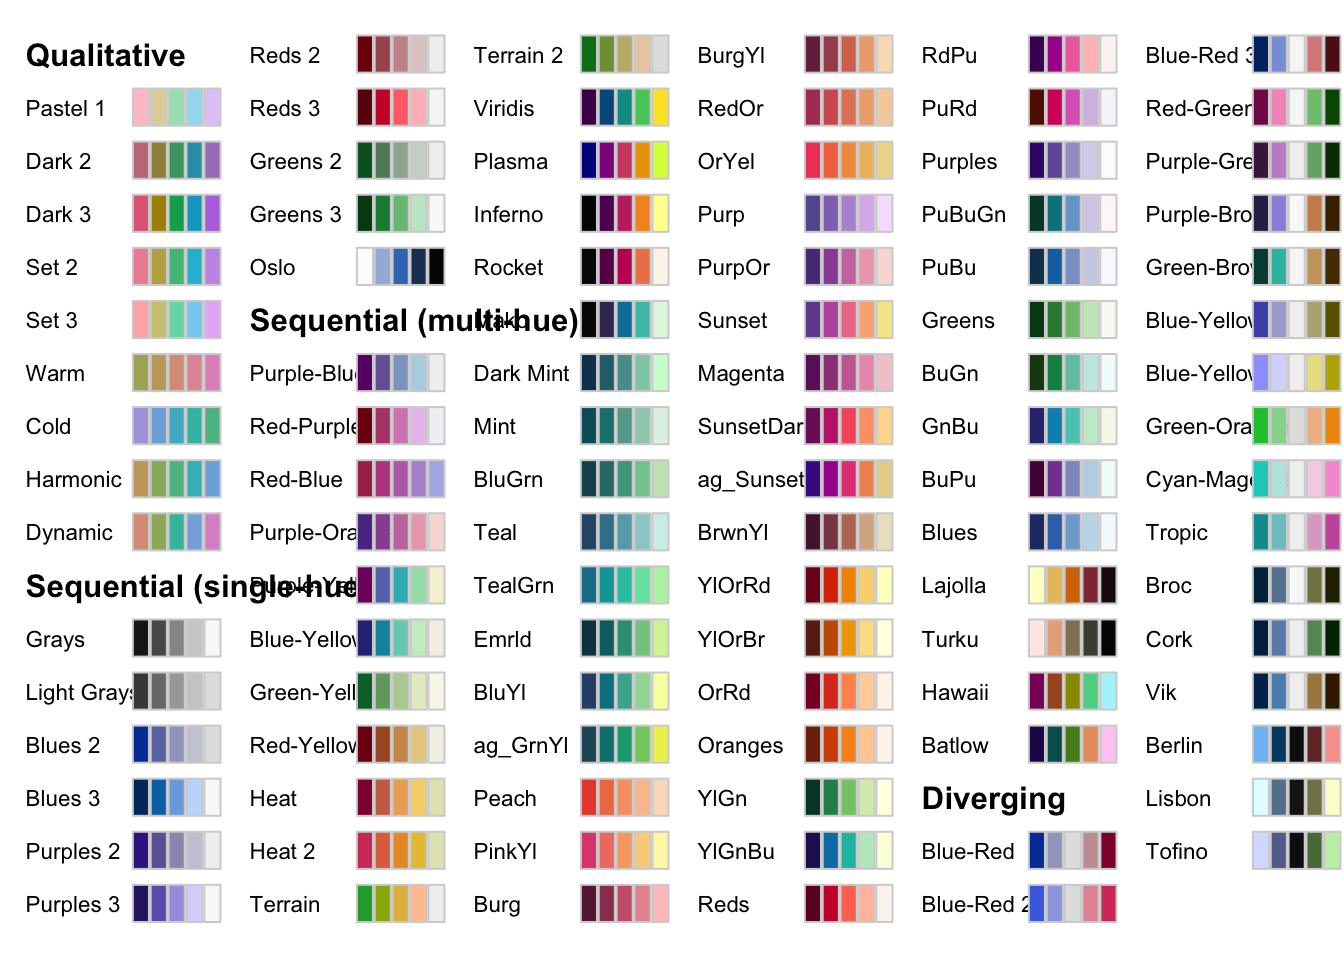
\includegraphics{Human-Centered-Data-Viz_files/figure-latex/chunk-label4-1-1.pdf}

However, our color vision is limited \citep{Johnson2014designingwiththemind}. Our visual system is much more sensitive to differences in color and brightness, i.e., to contrasting colors and edges, than to absolute brightness levels. We perceive colors not in absolute terms (see three types of cones) but as the difference between the color we are focusing on and the color that surrounds it \citep{Few2009nowtoseeit}. Our vision is therefore heavily impacted by the context.

There are three factors that affect our ability to distinguish colors from each other \citep{Johnson2014designingwiththemind}. First, the paler (less saturated) two colors are, the harder it is to tell them apart. Second, the the smaller or thinner objects are, the harder it is to distinguish their colors. Text is often thin, so the exact color of text is often hard to determine. Finally, the more separated color patches are, the more difficult it is to distinguish their colors, especially if the separation is great enough to require eye motion between patches.

But there are also external factors that influence how we can distinguish colors. Those factors are among others: the variation among color displays, gray-scale displays, display angle, and ambient lighting. These external factors are usually beyond your control but you should keep them in mind. Colors that appear distinguishable on your screen may not be so distinguishable in some of the environments in which the software is used.

A last issue you should consider is color blindness. Actual this term is mislabeled. It is not blindness, but rather a lack of color vision. It is the inability (or sometimes diminished ability) to see certain colors or perceive color contrasts in normal light. Color blindness is usually genetic, but in some cases it can be caused by disease or age. Furthermore, one in 12 men is color blind, compared to one in 200 women. The most common form of color blindness is red/green color blindness (protanopia). There are other, less common forms of color blindness that also involve different color pairs but also rare forms where colors can not be distinguished at all (achromatopsia).

To avoid that people cannot interpret your data visualizations correctly, you should use services such as \href{https://colorbrewer2.org}{ColorBrewer}. It supports you to select an appropriate color scheme by considering various user-selected criteria, including colorblind-friendliness.

\hypertarget{spation-vision}{%
\subsection{Spation Vision}\label{spation-vision}}

The spatial resolution of the human visual field drops greatly from the center to the edges. In the center 1\% of your visual field, i.e., the fovea, you have a high-resolution TIFF, and everywhere else, you have only a low-resolution JPEG. There are three reasons for this \citep{Johnson2014designingwiththemind}:

\begin{itemize}
\tightlist
\item
  Pixel density. Each eye has 6 to 7 million retinal cone cells. They are packed much more tightly in the fovea. The fovea has about 158,000 cone cells in each square millimeter. The rest of the retina has only 9,000 cone cells per square millimeter.
\item
  Data compression. Cone cells in the fovea connect 1:1 to the ganglial neuron cells that begin the processing and transmission of visual data, while elsewhere on the retina, multiple photoreceptor cells (cones and rods) connect to each ganglion cell. In technical terms, information from the visual periphery is compressed (with data loss) before transmission to the brain, while information from the fovea is not.
\item
  Processing resources. The fovea is only about 1\% of the retina, but the brain's visual cortex devotes about 50\% of its area to input from the fovea. The other half of the visual cortex processes data from the remaining 99\% of the retina.
\end{itemize}

The result is that our vision has much, much greater resolution in the center of our visual field than elsewhere. If our peripheral vision has such low resolution, why do we see our surroundings sharply and clearly?

We experience this illusion because our eyes move rapidly and constantly about three times per second even when we don't realize it, focusing our fovea on selected pieces of our environment. Our brain fills in the rest in a gross, impressionistic way based on what we know and expect. Our brain does not have to maintain a high-resolution mental model of our environment because it can order the eyes to sample and resample details in the environment as needed. We need this insights when we talk in the Chapter Interaction (Section \ref{sec:interaction}).

\hypertarget{pre-attentive-processing}{%
\section{Pre-Attentive Processing}\label{pre-attentive-processing}}

Many visual channels provide pre-attentive processing, where a distinct item stands out from many others immediately. The great value of preattentive processing is that the time it takes us to detect the different object does not depend on the number of distractor objects. Our low-level visual system performs massive parallel processing on these visual channels without requiring the viewer to consciously pay direct attention to the individual elements. Pre-attentive processing occurs for many channels. Examples are tilt, size, shape, proximity, and even shadow direction, but also various types of motion such as flicker, motion direction, and motion speed. However, a small number of potential channels do not support pre-attentive processing. One example is parallelism. Most visual channel pairs do not support pre-attentive processing, but some pairs do: one example is space and hue, and another is motion and shape. Pre-attentive processing is definitely not possible with three or more channels.

A question is, how we can systematically approach pre-attentive processing. Two principles can guide the use of visual channels in visual encoding: expressiveness and effectiveness. A set of facts that is \emph{expressible} in a visual language if the sentences (i.e.~the visualizations) in the language express all the facts in the set of data, and only the facts in the data. A visualization is more \emph{effective} than another visualization if the information conveyed by one visualization is more readily perceived than the information in the other visualization.

The expressiveness principle dictates that the visual encoding should express all of, and only, the information that the dataset exhibits. For example, ordered data (nominal) should be shown in a way that our perceptual system intrinsically senses as ordered and unordered data (ordinal) should not be shown in a way that perceptually implies an ordering. The expressiveness principle is especially important, wenn we talk about ethics in data visualization (Section \ref{sec:ethics})

The effectiveness principle dictates that the importance of the attribute should match the salience of the channel, i.e.~its noticeability. We already talked about colors but there are more visual channels we can consider when we decide about the visual encoding. The first researcher who thought about the effectiveness of visualizations is \href{https://en.wikipedia.org/wiki/Jacques_Bertin}{Jacques Bertin}.

\hypertarget{choice-of-encoding---bertins-guidance}{%
\subsection{Choice of Encoding - Bertin's Guidance}\label{choice-of-encoding---bertins-guidance}}

In 1967, Jacques Bertin published the book ``Semiologie Graphique'' (in English ``Semiology of Graphics'') that was based on his long-standing experience as a cartographer and geographer. In this book, Bertin linked human perception to visualization. Even though, this linking was more based on intuition than vision research, Bertin's experiences were later empirically proven. Bertin's key concept is the image, which is is the fundamental perceptual unit of a visualization. An ideal visualizations will contain only a single image in order to optimize ``efficiency,'' the speed with which observer can extract the information.

Bertin identified in his work that every visualization is made by a series of basic components that have different expressive power and that each one works best only in some conditions. In general, the encoding of data can be done in a coordinate system with the cartesian coordinate system as its most prominent representative. Of course, there are further coordinate systems, such as geographical coordinate system, parallel coordinates system, polar coordinate system, or the network coordinate system. Based on the chosen coordinate system, you need to place your data, more precisely your data values (e.g., items, links) into these coordinates. For this, you can differentiate so-called \emph{marks}. A mark is a basic graphical element which can be classified according to the number of spatial dimensions they require \citep{munzner2014visualization}: Possible dimensions are: a zero-dimensional (0D) mark is a point, a one-dimensional (1D) mark is a line, a two-dimensional (2D) mark is an area, a three- dimensional (3D) mark defines a volume.

\begin{figure}

{\centering 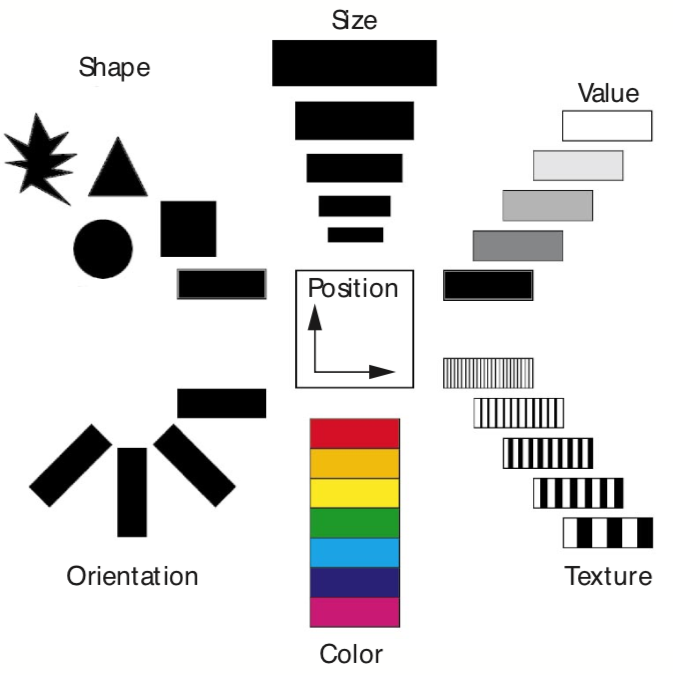
\includegraphics[width=0.5\linewidth]{images/bertin_visualattributes} 

}

\caption{Bertin’s Visual Channels Taken from McDonald (1999).)}\label{fig:unnamed-chunk-9}
\end{figure}

A visual channel defines the appearance of \emph{marks} (points, lines, areas), independent its dimensionality. Bertin differentiated six visual channels: size, value, texture, color, orientation, shape. For each of these channels he pointed out in what cases they work best and how to use them (cp.~Figure XX, redrawn from \citep{MacDonald1999usingcolor}). We already discussed that the human eye is independently sensitive to these visual channels, which means that more than one visual channel can be deployed at the same time in order to encode different variation in the data.

These visual channels can represent different relationships between marks:

\begin{itemize}
\tightlist
\item
  association (\(\equiv\)): the marks an be perceived as similar (\emph{group}),
\item
  selection (\(\ncong\)): the marks are perceived as different, forming families (\emph{distinguish}),
\item
  order (\(O\)): the marks are perceived as ordered (\emph{sort}), and
\item
  quantity (\(Q\)): the marks are perceived as proportional to each other (\emph{count}).
\end{itemize}

These perceptional properties can be arranged into the levels of organization \citep{green1998toward}. Associative perception is the lowest level of organization. It allows grouping all elements of a variable in spite of different values. `'Selective perception'' is the next higher level (flip side of association). It permits the viewer to select one category of a component, perceive locations of objects in that category and ignore others. Order allows the data to be ordinally ranked. An observer can see that one value of a variable represents a larger or smaller quantity than another. Quantity permits direct extraction of ratios, without need of consulting a legend, etc.

As said, Bertin's research has been empirically substantiated. Most notable are perhaps Cleveland and McGill's controlled experiments \citep{ClevelandMcGill1984graphicalperception}. The most important findings is that they mapped human response directly to visually encoded abstract information and provide explicit rankings of perceptual accuracy for each channel type.

Based on this work, Mackinlay \citep{Mackinlay1986automatingdesign} has derived perceptually-motivated rankings of the effectiveness of variables such as position, length, area, and color for encoding quantitative data. Heer and Bostock \citep{HeerBostock2010crowdsourcing} confirmed and extended this work through crowdsourcing. The only discrepancy is that the later research found length and angle judgments that are roughly equivalent.

\begin{figure}

{\centering 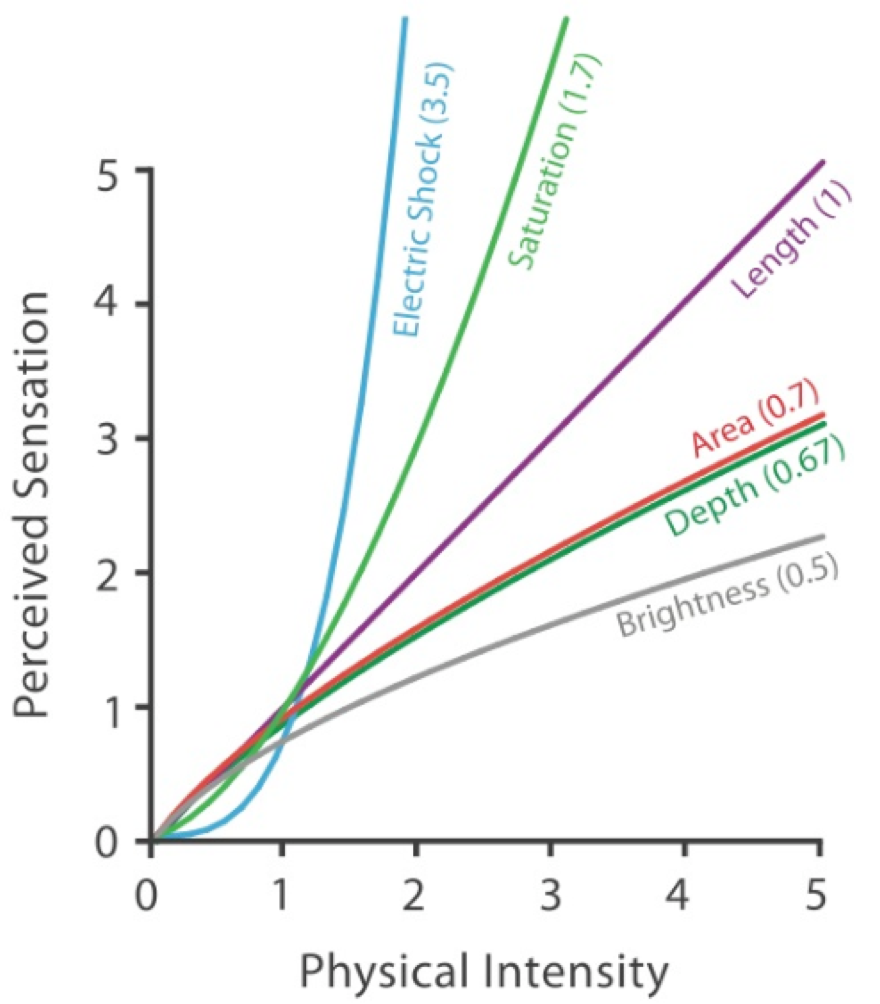
\includegraphics[width=0.5\linewidth]{images/stevens_psychophysicalpowerlaw} 

}

\caption{Results of Psychophysical power law of Stevens. Taken from Munzner (2014).)}\label{fig:unnamed-chunk-10}
\end{figure}

Their results for visual encodings agree well with psychophysical channel measurements. Psychophysics is devoted to the systematic measurement of general human perception \citep{StevensMarks2017Psychophysics}. We perceive different visual channels with different degrees of accuracy; they are not all equally distinguishable. Our responses to the sensory experience of size can be characterized by power-law/power-law, where the exponent depends on the precise sensory modality: Most stimuli are magnified or compressed; few remain unchanged. The diagram in Figure XX shows that length has an exponent of n = 1.0, so our perception of length is very close to the true value. Length means the length of a line segment on a 2D plane perpendicular to the observer. The other visual channels are not perceived as accurately: Area and brightness are compressed, while color saturation or electroshocks are magnified.

\hypertarget{combining-channels}{%
\section{Combining Channels}\label{combining-channels}}

Multiple visual channels can be combined to redundantly encode the same attribute. The limitation of this approach is that more channels are `'consumed'' so not as many attributes can be encoded in total, but the advantage is that the attributes represented are very well perceived.

However, visual channels are not completely independent of each other, since some have dependencies and interactions with others \citep{munzner2014visualization}. You must consider a continuum of potential interactions between channels for each pair, ranging from orthogonal and independent separable channels to inseparably combined integrated channels. Visual encoding is straightforward for single channels, but attempts to encode different information in integrated channels will fail. People will not be able to access the desired information about each attribute, but an unexpected combination will be perceived.

\emph{Separability of Visual Channels}: A pair of channels that are completely separable is position and hue.
An example of interference between the channels, showing that size is not completely separable from hue. Size interacts with many visual channels, including shape.
Integral pair is an encoding of one variable with horizontal size and another with vertical size. It is ineffective because what we perceive directly is the planar size of the circles, namely their area.
An inseparable pair of channels is the red and green channels of the RGB color space. These channels are not perceived separately, but are integrated into a combined color perception, so the three channels are not perceptual.

\emph{Grouping of Visual Channels}:
The encoding of link markers using containment/containment or link lines conveys the information that the linked objects form a group with a very strong perceptual cue. Containment is the strongest cue for grouping, with linkage a close second.
Another way to convey that elements form a group is to encode categorical data according to identity channels. All elements that share the same level of categorical attribute can be perceived as a group simply by selectively directing attention to that level. The perceptual grouping cue of identity channels is not as strong as using link or containment markers, but one advantage of this lightweight approach is that it does not add additional clutter in the form of extra link markers.
The third strongest grouping approach is proximity, which is the placement of objects within the same spatial region. This phenomenon of perceptual grouping is the reason why the best placed channel for encoding categorical data is a spatial region.
The final grouping channel is the similarity to the other categorical channels of hue and motion, and also shape if carefully selected. Logically, proximity is like similarity for spatial position; however, from a perceptual perspective, the effect of the spatial channels is so much stronger than the effect of the others that it makes sense to consider them separately.

\hypertarget{visualizing-tabular-data}{%
\chapter{Visualizing Tabular Data}\label{visualizing-tabular-data}}

Now you learnt about the general process of creating data visualizations and we have also discussed certain restrictions that exist in human visual and spatial cognition. These foundations help us to dive deeper into the topic of visualizations. In the next three chapters, we explore various visualizations and their characteristics. This helps you to make an informed decision when selecting for a certain visual encoding.

The majority of ``found'' data is available in a tabular format, since it is very convenient for understanding and working with the data. In this chapter, thus, we focus on this data type.

Tabular data \citep{munzner2014visualization} consists of key (often the header) and value attributes. A key is an independent attribute that can be used as a unique index to look up items in a table. It can be a categorical or ordinal variable. A value is a dependent attribute: the value of a cell in a table. Values can be categorical, ordinal, or quantitative attributes. What are our possibilities for transferring tabular data into a certain visual encoding? Our decision depends on the semantics of the table's attributes, i.e., how many keys and how many values our table has. In case of two value attributes that are quantitative, we can use a scatterplot, with one key (categorical) and one value attribute (quantitative), a bar chart is appropriate, and heatmaps show two keys (categorial) and one value (quantitative). In the following sections, we explore possible visual encodings in more detail by focusing on four aspects \citep{munzner2014visualization}:

\begin{itemize}
\tightlist
\item
  Visual Encoding for Numerical Data
\item
  Visual Encoding for Categorical Data
\item
  Spatial Axis Orientation
\item
  Spatial Layout Density
\end{itemize}

\hypertarget{visual-encoding-for-numerical-data}{%
\section{Visual Encoding for Numerical Data}\label{visual-encoding-for-numerical-data}}

As you already know, quantitative attributes, i.e., numerical data, can visually be encoded by representing them over the spatial position channel. The most simple representation is to encode a single quantitative attribute along an axis by encoding each element of the attribute with a marker. When you have two quantitative attributes you use the \textbf{scatterplot} by encoding the values on the vertical and horizontal spatial position channels, respectively. The mark type is necessarily a point and additional attributes can be encoded with other non-spatial channels such as color and size. Size-coded scatterplots are sometimes referred to as \textbf{bubble charts}.

As discussed in the EDA Chapter \ref{Understanding-the-Data-Structure} scatter plots are useful for characterizing distributions, especially for finding outliers and extreme values. They are also very effective for assessing the correlation between the two attributes.

An example for an appropriate usage of an scatterplot (with animation) is the \emph{Trend-Analyzer} \citep{Robertsonetal2008trendanalyzer}. The scatterplot uses additional attributes, such as color and size coding of marks. The \emph{Trend-Analyzer} uses demographic data of infant mortality against life expectancy. Each dot marker represents a country whose horizontal and vertical spatial positions encode the life expectancy and infant mortality. The color channel is used for the categorical country attribute and the size channel for the quantitative population attribute.

However, besides the encoding of the data, scatterplots have so-called non-data components, such as axes and legends. These components are often just as important as the data itself since they provide contextual information for interpreting the data \citep{Talbotetal2010ticklabels}. The labeling of the axis, for example, allows the viewer to lookup values, to mentally compute ranges, or to estimate the slope. Over the years, many researchers of thought of approaches to algorithmically create `'nice'' labels (such as ). Discussing these approaches is beyond the scope of this lecture but I want to highlight one research work by Talbot et al. \citep{Talbotetal2010ticklabels}. They compared different approaches in this sphere and recommended a new search algorithm for finding an optimal labeling for a given dataset. This algorithms considers the following components:

\begin{enumerate}
\def\labelenumi{\arabic{enumi}.}
\tightlist
\item
  Simplicity, i.e., the numbers of the tick marks should be multiples of 10, 5, 2
\item
  Coverage, i.e., there should be tick marks close to the ends of the data
\item
  Density, i.e., there should not too many, nor too few tick marks.
\item
  Legibility, i.e., the formatting of the label (e.g., 5M vs.~5,000,000), font size (e.g., for avoiding overlapping labels), and orientation (e.g., o handle extremely dense axis) should be considered.
\end{enumerate}

However, an automatic axis labeling is just one component to think of in (automated) graphic design. Such considerations should also include the layout of an entire plot, including the placement of titles, axis titles, legends, data labels, or aspect ratio (via banking to \(45^{\circ}\)). We talk about the latter in more detail in Section \ref{Visual-Encoding-for-Categorical-Data}.

Another important decision in graphic design is the issue of axis scaling. One question that is discussed in literature is whether scaling to zero is necessary. On the one hand `'zooming in'' helps to understanding the differences in the data, bot on the other hand, it can be misleading. The decision depend on the visual encoding of the data. Bar charts, for example, use position (end of bar) and size (length and area) to encode numeric values. When `'zooming in'' bar chats, the length of a bar encodes meaningless information. In any case, when you do not start you graph with a zero-based scale, make sure that your inform the reader about this design decision.

Another challenge occurs if the data is very unevenly distributed. Imagine you have data where the majority of data is very close together but there is one outlier. Because of this outlier, the majority of data is compressed and individual differences are challenging to be caught. What can you do? Well, the easiest the most straightforward approach might be to skip the outlier, however, in many cases such data manipulation is not appropriate. There are two approaches that can help to overcome this discussed challenge: the use of a scale break and the transformation of the data (by using a logarithmic scale).

Scale break should be designed with care. Conventional scale breaks consists of two short parallel lines intersecting the axis. Such scale breaks should be avoided since often the viewer of the graph may overlook this important information. However, there is also the so-called full scale break which divides the graph into two panels, each with a full frame and its own scale \citep{Cleveland1984fullscalebreaks}. The visual discontinuity discourages pattern or continuity perception across the break. However, the more frequently applied strategy is data transformation by using a log scale. Both approaches increase the visual resolution of the data. The scale break makes it difficult to compare the data, since you have to cognitively and not perceptually consume the data. As opposed to the log scale, where you can directly compare all data.

Logarithmic Transformation of data has many advantages, since you can address data skew, for example, when having a long tail or outliers. It enables the viewer the comparison within and across multiple orders of magnitude. However, you have to consider how the logarithmic transformation works. The transformation focuses on multiplicative (not additive) factors. You have percentage change and not a linear difference. However, in two cases you should avoid using a log scale: when you have negative non-zero values and when you audience is potential not familiar with this type of scale transformation (which is rather the rule rather than the exception).

\hypertarget{Visual-Encoding-for-Categorical-Data}{%
\section{Visual Encoding for Categorical Data}\label{Visual-Encoding-for-Categorical-Data}}

The use of space to encode categorical attributes is a bit more complex, since categorical attributes have often a disordered semantics. Remember, the principle of expressivity would be violated if categorical attributes are encoded using spatial position \citep{munzner2014visualization}.

Drawing all of the items with the same values for a categorical attribute within the same region uses spatial proximity to encode the information about their similarity. The regions themselves must be given spatial positions on the plane in order to draw any specific picture. The distribution of regions can be divided into three operations: separating into regions, aligning the regions, and ordering the regions. The separation should be done according to an attribute that is categorical, whereas alignment and ordering should be done by some other attribute that can be ordered.

We already talked about the simple \textbf{bar chart} that are suitable if your tabular data consisting of one numerical and one categorial attribute. You use line marks to express the value attribute with aligned vertical position and you separate the key attribute with horizontal position. Bar chart support the lookup of values or their comparison. They scale well up to dozens to hundreds of key attributes.

Another often used bar chart tye is the \textbf{grouped bar chart} if you have one numerical and a number of categorical attributes.

What we often see are \textbf{stacked bar charts} \citep{munzner2014visualization}. The scalability of stacked bar charts is similar to that of standard bar charts in terms of the number of categories in the key attribute distributed across the major axis, but is limited for the key used to stack. This idiom works well with multiple categories, with an upper limit of about a dozen. A normalized stacked bar chart stretches each of these bars to the maximum possible length and shows percentages rather than absolute values. Only the lowest subbar in a stacked bar chart is aligned with the others in its category, so that the most accurate position channel can be used with respect to a common frame. The other subbars use an unaligned position, a channel that is less accurate than the aligned position, but still more accurate than angle comparisons. If used stacked bar charts should allow the viewer to interactively change the order.

Both, the simple, grouped, and stacked bar chart can often be replaced by a \textbf{dot chart}. This chart has a number of advantages compared to other more widely used visualizations, such as the bar chart \citep{Soenning2016dotplot}. The dot plot was introduced by Cleveland \citep{ClevelandMcGill1984graphicalperception}. The horizontal scale encodes a quantitative variable and the vertical scale a categorical variable. Furthermore, light horizontal lines connect the data points with their labels.

Another often use diagram you know already of a \textbf{line charts}. A line chart has one quantitative attribute and one order attribute. Line charts often emphasize trend relationships. Zacks and Tversky \citep{ZacksTversky1999linechartbarchart}, for example, studied how people answered questions on the categorical data type gender compared to the quantitative data type age, as shown in the figure. Line graphs for quantitative data provided appropriate trend-related answers, such as ``height increases with age.'' Bar charts for quantitative data yielded equally appropriate discrete comparison responses, such as ``Twelve-year-olds are taller than ten-year-olds.'' However, line graphs for categorical data yielded inappropriate trend responses such as ``The more male a person is, the taller he is.'' This experiment emphasize the importance of well-chosen visual encodings.

However, the same data can look very different in a line chart depending on its aspect ratio. But what is the perfect shape for a chart? The ratio between the width and height of a rectangle is called the aspect ratio. It is typically expressed as a fraction with two numbers, where the width is divided by the height. An aspect ratio of 1:1 describes a square, while 4:3 (or 1.33:1) is a landscape rectangle and 16:9 is a much wider landscape rectangle. While width is usually greater than height in film and photography, there is no reason for this to be the case in visualization. Short answer is: `'It depends on the data.''. However, Cleveland et al. \citep{ClevelandMcGill1984graphicalperception} proposed the idea that the average line slope in a line chart should be \(45^{\circ}\). This was called banking to \(45^{\circ}\) and has become one of the bits of common wisdom in visualization that determines the ideal aspect ratio. In other words, a rule of thumb is that the average line inclination in a line chart should be 45 degrees. Heer and Agrawala \citep{HeerAgrawala2006banking} extended this approach, by analyzing data for trends at various frequency scales and then generates a banked chart for each of these scales.

The aforementioned visualization are suitable for less complex data sets, but what do you do, if this is not the case. Two visualization that you should take in mind a the heatmap and the scatterplot matrix.

A \textbf{heatmap} is used to encode two categorical and one quantitative attribute \citep{munzner2014visualization}. It is suitable for finding cluster, outliers, and to summarize data. The advantage of heat maps is that the visual coding of quantitative data with color using small area markers is very compact, making them well suited for overviews with high information density. An extension is the \textbf{cluster heat map}, it is the side-by-side combination of a heat map and two dendrograms that display the derived data from the cluster hierarchies used in the matrix reordering. The goal of this reordering is to group similar cells together to look for patterns between the two attributes.

A \textbf{scatterplot matrix} (SPLOM) is a matrix where each cell contains an entire scatterplot diagram \citep{munzner2014visualization}. A SPLOM shows all possible pairwise combinations of attributes, using the original attributes as rows and columns. Unlike the simple heatmap matrix where each cell displays an attribute value, an SPLOM is an example of a more complex matrix where each cell displays a complete graph. SPLOMs are heavily used for the abstract tasks of finding correlations, trends, and outliers, according to the use of their constituent scatter plot components.

\hypertarget{spatial-axis-orientation}{%
\section{Spatial Axis Orientation}\label{spatial-axis-orientation}}

In a rectilinear layout, regions or elements are distributed along two orthogonal axes, the horizontal and vertical spatial positions, ranging from a minimum value on one side of the axis to a maximum value on the other. Rectilinear layouts are heavily used in vis design and appear in many common statistical charts. All examples discussed so far used rectilinear layouts. However, the spatial axes alignment as another design option in visualization design, thus, you have choices. You can use for your spatial axes a rectilinear, parallel or radial layout \citep{munzner2014visualization}.

An example for the parallel layout are \textbf{parallel coordinates}. It is an approach for visualizing many quantitative attributes at once using spatial position. As the name suggests, the axes are placed parallel to each other, rather than orthogonal at right angles.
In parallel coordinates a single item is represented by a jagged line that zigzags through the parallel axes, crossing each axis exactly once at the location of the item's value for the associated attribute. Parallel coordinates scale to show hundreds of elements, but not thousands. If too many lines are overdrawn, the resulting occlusion provides very little information. Original motivation of parallel coordinates was that they are used to check for correlations between attributes. When two adjacent axes have a high positive correlation, the line segments are mostly parallel. When two axes have a high negative correlation, the line segments usually cross at a point between the axes. The pattern between uncorrelated axes is a mixture of crossing angles. In practice, however, SPLOMs are typically easier to use to find a correlation. Parallel coordinates are used to get an overview of all attributes, to classify the range of values of attributes, to select a range of elements or to detect outliers.

In a radial spatial layout, elements are distributed around a circle using the angular channel in addition to one or more linear spatial channels, as opposed to rectilinear layouts which use only two spatial channels. The natural coordinate system in radial layouts is \textbf{polar coordinates}, where one dimension is measured as an angle from a starting line and the other as a distance from a center point. Radial layouts can be more effective than rectilinear in representing the periodicity of patterns, however, encoding non-periodic data with the periodic channel of the angle can be misleading. Radial layouts imply an asymmetry of meaning between the two attributes and would be inappropriate if the two attributes have the same meaning.

The most commonly used radial statistical graph is the \textbf{pie chart}. It encodes a single attribute with area markers and the angle channel. Despite their popularity, pie charts are clearly problematic. Angle judgments at area markers are less accurate than length judgments at line markers. Wedges vary in width along the radial axis, from narrow near the center to wide near the outside, making area judgments particularly difficult.

The most useful property of pie charts is that they show the relative contribution of parts to a whole. The sum of the wedge angles must add up to \(360^{\circ}\) of a full circle and match normalized data, such as percentages where the parts must add up to 100\%. However, this property is not only important for pie charts; a single bar in a normalized stacked bar chart can also be used to indicate this property with the more accurate length assessment channel.

\hypertarget{spatial-layout-density}{%
\section{Spatial Layout Density}\label{spatial-layout-density}}

Another design choice with spatial visual coding ideas is whether a layout is dense or sparse.

A dense (pixel oriented) layout uses small and densely packed marks to provide an overview of as many items as possible with very high information density. A maximally dense layout has point marks that are only a single pixel in size and line marks that are only a single pixel in width. The small size of the marks implies that only the planar position and color channels can be used in visual encoding.

A space-filling layout has the property that it fills all available space in the view, as the name implies. Space-filling layouts typically use area marks for items or containment marks for relationships, rather than line or connection marks, or point marks. An advantage of space-filling approaches is that they maximize the space available for color markings. On the other hand, a disadvantage of space-filling views is that the designer cannot use white space in the layout. Many graphic design guidelines refer to the careful use of white space for many reasons, including legibility, emphasis, relative importance, and visual balance. Space-filling layouts usually strive for a high density of information. However, the characteristic that a layout fills space is by no means a guarantee of efficient use of space. Technically, the definition of space filling is that the total area used by the layout is equal to the total area available in the view. An example of a space-filling layout are \href{treemap}{treemaps} which are discussed in the next chapter.

  \bibliography{book.bib,packages.bib}

\end{document}
